% ------------------------------------------------------------------------
% ------------------------------------------------------------------------
% Modelo UFSC para Trabalhos Academicos (tese de doutorado, dissertação de
% mestrado) utilizando a classe abntex2
%
% Autor: Alisson Lopes Furlani
% 	Modificações:
%	- 27/08/2019: Alisson L. Furlani, add pacote 'glossaries' para listas
%   - 06/11/2019: Luiz-Rafael Santos, modifica para Trabalho de Conclusão de Curso
% ------------------------------------------------------------------------
% ------------------------------------------------------------------------

\documentclass[
	% -- opções da classe memoir --
	12pt,				% tamanho da fonte
	%openright,			% capítulos começam em pág ímpar (insere página vazia caso preciso)
	oneside,			% para impressão no anverso. Oposto a twoside
	a4paper,			% tamanho do papel. 
	% -- opções da classe abntex2 --
	chapter=TITLE,		% títulos de capítulos convertidos em letras maiúsculas
	section=TITLE,		% títulos de seções convertidos em letras maiúsculas
	%subsection=TITLE,	% títulos de subseções convertidos em letras maiúsculas
	%subsubsection=TITLE,% títulos de subsubseções convertidos em letras maiúsculas
	% -- opções do pacote babel --
	%english,			% idioma adicional para hifenização
	%french,				% idioma adicional para hifenização
	%spanish,			% idioma adicional para hifenização
	brazil				% o último idioma é o principal do documento
	]{abntex2}

\usepackage{setup/ufscthesisA4-alf}
\usepackage{amssymb}

% ---
% Filtering and Mapping Bibliographies
% ---
% Pacotes de citações
% ---
\usepackage{csquotes}
\usepackage[backend = biber, style = abnt]{biblatex}
% FIXME Se desejar estilo numérico de citações,  comente a linha acima e descomente a linha a seguir.
% \usepackage[backend = biber, style = numeric-comp]{biblatex}


%\usepackage{color} %permite o uso de cores no documento
%\usepackage[table]{xcolor}
%\usepackage{framed} %%allows to use background color in the table box


% Pacotes usados especificamente neste documento
\usepackage{graphicx} % Possibilita o uso de figuras e gráficos
\usepackage{color}    % Possibilita o uso de cores no documento
\usepackage{listings}
\usepackage{multirow}
\usepackage{tabularx}
\usepackage[table]{xcolor}
\usepackage{colortbl}
\usepackage{framed}
\usepackage{float}
%\usepackage{footnote}
%\makesavenoteenv{tabular}
%\makesavenoteenv{table}
%\usepackage[printonlyused, withpage]{acronym}
\usepackage{pdfpages}
\usepackage{afterpage}
\usepackage{hhline}
\usepackage{enumitem}
\usepackage{latexsym}
\usepackage{svg}
\usepackage{amsmath}
\usepackage{multirow}
%\usepackage{bm}
%\usepackage{amssymb}
\usepackage[lined,boxed,ruled,commentsnumbered,portuguese]{algorithm2e}

\usepackage{lipsum}

\definecolor{shadecolor}{rgb}{0.8,0.8,0.8}

\setlength\bibitemsep{\baselineskip}
\DeclareFieldFormat{url}{Disponível~em:\addspace\url{#1}}
\NewBibliographyString{sineloco}
\NewBibliographyString{sinenomine}
\DefineBibliographyStrings{brazil}{%
	sineloco     = {\mkbibemph{S\adddot l\adddot}},
	sinenomine   = {\mkbibemph{s\adddot n\adddot}},
	andothers    = {\mkbibemph{et\addabbrvspace al\adddot}},
	in			 = {\mkbibemph{In:}}
}

\addbibresource{aftertext/references.bib} % Seus arquivos de referências

% ---
\DeclareSourcemap{
	\maps[datatype=bibtex]{
		% remove fields that are always useless
		\map{
			\step[fieldset=abstract, null]
			\step[fieldset=pagetotal, null]
		}
		% remove URLs for types that are primarily printed
%		\map{
%			\pernottype{software}
%			\pernottype{online}
%			\pernottype{report}
%			\pernottype{techreport}
%			\pernottype{standard}
%			\pernottype{manual}
%			\pernottype{misc}
%			\step[fieldset=url, null]
%			\step[fieldset=urldate, null]
%		}
		\map{
			\pertype{inproceedings}
			% remove mostly redundant conference information
			\step[fieldset=venue, null]
			\step[fieldset=eventdate, null]
			\step[fieldset=eventtitle, null]
			% do not show ISBN for proceedings
			\step[fieldset=isbn, null]
			% Citavi bug
			\step[fieldset=volume, null]
		}
	}
}
% ---

% ---
% Informações de dados para CAPA e FOLHA DE ROSTO
% ---
% FIXME Substituir 'Nome completo do autor' pelo seu nome.
\autor{Samuel Moreira Ransolin}
% FIXME Substituir 'Título do trabalho' pelo título da trabalho.
\titulo{Detecção de Documentos Acadêmicos Falsificados: Uma Solução Baseada em Aprendizado de Máquina}%Circuit optimization with routing with Cell movement %using the OpenROAD project infrastructure }
% FIXME Substituir 'Subtítulo (se houver)' pelo subtítulo da trabalho.  
% Caso não tenha substítulo, comente a linha a seguir.
%\subtitulo{Subtítulo (se houver)}
% FIXME Substituir 'XXXXXX' pelo nome do seu
% orientador.
% \orientador{XXXXXXX, Dr.}
% FIXME Se for orientado por uma mulher, comente a linha acima e descomente a linha a seguir.
\orientador[Orientadora]{Giovana Nunes Inocêncio, M.a.}
% FIXME Substituir 'XXXXXX' pelo nome do seu
% coorientador. Caso não tenha coorientador, comente a linha a seguir.
\coorientador[Coorientador]{Prof. Jean Everson Martina, Dr.}
% FIXME Se for coorientado por uma mulher, comente a linha acima e descomente a linha a seguir.
\coorientador{}
% FIXME Substituir 'XXXXXX' pelo nome do Coordenador do 
% programa/curso.
\coordenador{Profa. Lúcia Helena Martins Pacheco, Dr.}
% FIXME Se for coordenadora mulher, comente a linha acima e descomente a linha a seguir.
\bancaa{Giovana Nunes Inocêncio, M.a.}
\bancab{Prof. Jean Everson Martina, Dr.}
%\formacao{Engenheira de Controle e Automação}
\bancac{Lucas Machado da Palma, Dr.} %Primeiro membro da banca (normalmente o orientador).
\bancad{Gabriel Estevam de Oliveira, M.e.} %Segundo membro da banca
% \coordenador[Coordenadora]{Nome da Coordenadora, Dra.}
% FIXME Substituir '[ano da entrega]' pelo ano (ano) em que seu trabalho foi defendido.
\ano{2025}
% FIXME Substituir '[dia] de [mês] de [ano]' pela data em que ocorreu sua defesa.
\data{[11] de [12] de [2025]}
% FIXME Substituir '[Cidade da defesa]' pela cidade em que ocorreu sua defesa.
\local{Florianópolis}
\instituicaosigla{UFSC}
\instituicao{Universidade Federal de Santa Catarina}
% FIXME Substituir 'Dissertação/Tese' pelo tipo de trabalho (Tese, Dissertação). 
\tipotrabalho{Relatório de Trabalho de Conclusão de Curso 1}
% FIXME Substituir '[licenciado/bacharel] em [nome do título obtido]' pela grau adequado.
\formacao{Bacharel em Ciências da Computação}
% FIXME Substituir '[licenciado/bacharel]' pelo nivel adequado.
\nivel{Bacharel}
% FIXME Substituir 'Curso de Graduação em [XXXXXXXX]' pela curso adequado.
\programa{Curso de Graduação em Ciências da Computação}
% FIXME Substituir 'Campus XXXXXX ou Centro de XXXXXX' pelo campus ou centro adequado.
\centro{Centro Tecnológico}
\preambulo
{%
\imprimirtipotrabalho~do~\imprimirprograma~do~\imprimircentro~da~\imprimirinstituicao~para~a~obtenção~do~título~de~\imprimirformacao.
}
% ---

% ---
% Configurações de aparência do PDF final
% ---
% alterando o aspecto da cor azul
\definecolor{blue}{RGB}{41,5,195}
% informações do PDF
\makeatletter
\hypersetup{
     	%pagebackref=true,
		pdftitle={\@title}, 
		pdfauthor={\@author},
    	pdfsubject={\imprimirpreambulo},
	    pdfcreator={LaTeX with abnTeX2},
		pdfkeywords={ufsc, latex, abntex2}, 
		colorlinks=true,       		% false: boxed links; true: colored links
    	linkcolor=black,%blue,          	% color of internal links
    	citecolor=black,%blue,        		% color of links to bibliography
    	filecolor=black,%magenta,      		% color of file links
		urlcolor=black,%blue,
		bookmarksdepth=4
}
\makeatother
% ---

% ---
% compila a lista de abreviaturas e siglas e a lista de símbolos
% ---

% Declaração das siglas
% \siglalista{VLSI}{\textit{Very Large-Scale Integrated}}
% \siglalista{GRT}{\textit{Global Routing}}
% \siglalista{EDA}{\textit{Electronic Design Automation}}
% \siglalista{HDL}{\textit{Hardware Description Language}}
% \siglalista{RTL}{\textit{Register Transfer Level}}
% \siglalista{IC}{\textit{Integrated Circuit}}
% \siglalista{CAD}{\textit{Computer-Aided Design}}
% \siglalista{TCC}{\textit{Trabalho de Conclusão de Curso}}
% \siglalista{RCM}{\textit{Routing with Cell Movement}}
% \siglalista{DT}{\textit{Decision Trees}}
% \siglalista{NN}{\textit{Neural Network}}
% \siglalista{RMSE}{\textit{Root-Mean-Square Error}}
% \siglalista{R-squared}{\textit{Coefficient of determination}}
% \siglalista{DNN}{\textit{Deep Neural Network}}
% \siglalista{ASIC}{\textit{Application Specific Integrated Circuit}}
% \siglalista{ER}{\textit{Error Rate}}
% \siglalista{ED}{\textit{Error Distance}}
% \siglalista{PCB}{\textit{Printed Circuit Boards}}
% \siglalista{HPWL}{\textit{Half Perimeter Wirelength}}
% \siglalista{IP}{\textit{Intellectual Property}}
% \siglalista{MPSoC}{\textit{Multiprocessor System-on-Chip}}
% Declaração dos simbolos
% \simbololista{ci}{\ensuremath{c_i}}
% {Célula i}
% \simbololista{R}{\ensuremath{R}}{Conjunto das redes}
% \simbololista{Rci}{\ensuremath{R(c_i)}}{Conjunto das redes conectados à célula i}
% \simbololista{rk}{\ensuremath{r_k}}
% {Rede k}
% \simbololista{pi}{\ensuremath{\pi}}{Número pi} 
% \simbololista{r}{\ensuremath{r}}{Raio de um círculo}
% \simbololista{A}{\ensuremath{A}}{Área de um círculo}

% compila a lista de abreviaturas e siglas e a lista de símbolos
\makenoidxglossaries 

% ---

% ---
% compila o indice
% ---
\makeindex
% ---

% ----
% Início do documento
% ----
\begin{document}

% Seleciona o idioma do documento (conforme pacotes do babel)
% \selectlanguage{english}
\selectlanguage{brazil}

% Retira espaço extra obsoleto entre as frases.
\frenchspacing 

% Espaçamento 1.5 entre linhas
\OnehalfSpacing

% Corrige justificação
%\sloppy

% ----------------------------------------------------------
% ELEMENTOS PRÉ-TEXTUAIS
% ----------------------------------------------------------
% \pretextual %a macro \pretextual é acionado automaticamente no início de \begin{document}
% ---
% Capa, folha de rosto, ficha bibliografica, errata, folha de apróvação
% Dedicatória, agradecimentos, epígrafe, resumos, listas
% ---
% ---
% Capa
% ---
\imprimircapa
% ---

% ---
% Folha de rosto
% (o * indica que haverá a ficha bibliográfica)
% ---
\imprimirfolhaderosto*
% ---

% ---
% Inserir a ficha bibliografica
% ---
% http://ficha.bu.ufsc.br/
%\begin{fichacatalografica}
%	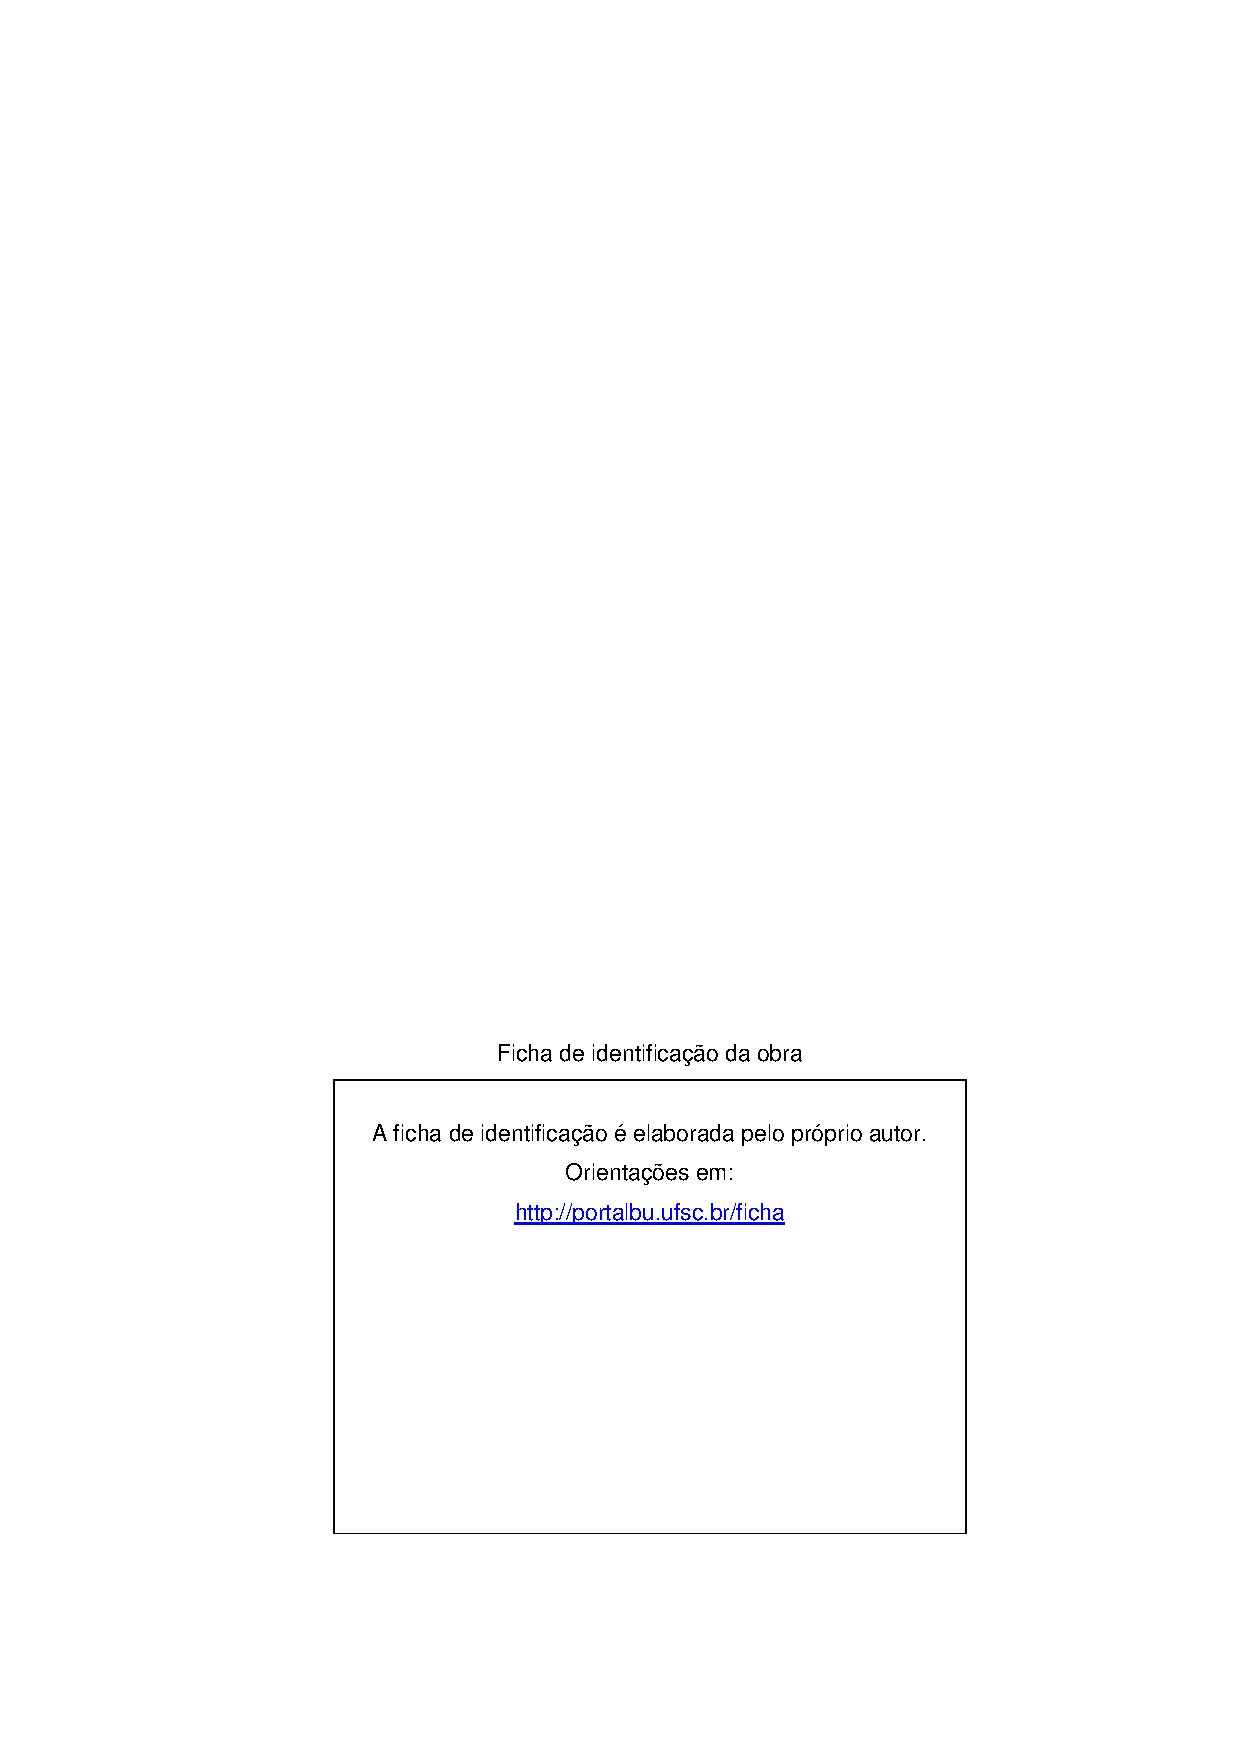
\includepdf{beforetext/Ficha_Catalografica.pdf}
%\end{fichacatalografica}
% ---

% ---
% Inserir folha de aprovação
% ---
%\begin{folhadeaprovacao}
	%\OnehalfSpacing
	%\centering
	%\imprimirautor\\%
	%\vspace*{10pt}		
	%\textbf{\imprimirtitulo}%
	%\ifnotempty{\imprimirsubtitulo}{:~\imprimirsubtitulo}\\%
	%		\vspace*{31.5pt}%3\baselineskip
	%\vspace*{\baselineskip}
	%\begin{minipage}{\textwidth}
	%% ~do~\imprimirprograma~do~\imprimircentro~da~\imprimirinstituicao~para~a~obtenção~do~título~de~\imprimirformacao.
	%Este~\imprimirtipotrabalho~foi julgado adequado para obtenção do Título de “\imprimirformacao” e aprovado em sua forma final pelo~\imprimirprograma. \\
	%	\vspace*{\baselineskip}
	%\imprimirlocal, \imprimirdata. \\
	%\vspace*{2\baselineskip}
	%\assinatura{\OnehalfSpacing\imprimircoordenador \\ %\imprimircoordenadorRotulo~do Curso}
	%\vspace*{2\baselineskip}
	%\textbf{Banca Examinadora:} \\
	%\vspace*{\baselineskip}
	%\assinatura{\OnehalfSpacing\imprimirorientador \\ %\imprimirorientadorRotulo}
%	%\end{minipage}%
%	\vspace*{\baselineskip}
%	\assinatura{Prof.(a) xxxx, Dr(a).\\
%	Avaliador(a) \\
%	Instituição xxxx}

%	\vspace*{\baselineskip}
%	\assinatura{Prof.(a) xxxx, Dr(a).\\
%	Avaliador(a) \\
%	Instituição xxxx}


%\end{folhadeaprovacao}

\begin{folhadeaprovacao}
	\OnehalfSpacing
	\centering
	\imprimirautor\\%
	\vspace{24pt}		
	\textbf{\imprimirtitulo}%
	\ifnotempty{\imprimirsubtitulo}{:~\imprimirsubtitulo}\\%
	%		\vspace*{31.5pt}%3\baselineskip
	\vspace*{\baselineskip}
	%\begin{minipage}{\textwidth}
	Este Trabalho de Conclusão de Curso foi julgado adequado para obtenção do Título de ``\imprimirformacao'' e aprovado em sua forma final pelo Curso de Graduação em Ciências da Computação.\\
	\vspace{12pt}
	\imprimirlocal, 11~de~dezembro~de~\imprimirano.\\
	
	\vspace*{18pt}
	\textbf{Banca Examinadora:}\\
	
	\vspace*{24pt}
	\assinatura{\OnehalfSpacing \imprimirbancaa}
	\vspace{6pt}
	Universidade Federal de Santa Catarina\\
	
	\vspace*{24pt}
	\assinatura{\OnehalfSpacing \imprimirbancab}
	\vspace{6pt}
	Universidade Federal de Santa Catarina\\
	
	\vspace*{24pt}
	\assinatura{\OnehalfSpacing \imprimirbancac}
	\vspace{6pt}
	Universidade Federal de Santa Catarina\\

    \vspace*{24pt}
	\assinatura{\OnehalfSpacing \imprimirbancad}
	\vspace{6pt}
	Universidade Federal de Santa Catarina\\
	
\end{folhadeaprovacao}

% ---

% ---
% Dedicatória
% ---
%\begin{dedicatoria}
%	\vspace*{\fill}
%	\noindent
%	\begin{adjustwidth*}{}{5.5cm}     
%		Este trabalho é dedicado aos meus colegas de classe e aos meus queridos pais.
%	\end{adjustwidth*}
%\end{dedicatoria}
% ---

% ---
% Agradecimentos
% ---
%\begin{agradecimentos}
%	Inserir os agradecimentos aos colaboradores à execução do trabalho. 
	
%	Xxxxxxxxxxxxxxxxxxxxxxxxxxxxxxxxxxxxxxxxxxxxxxxxxxxxxxxxxxxxxxxx. 
%\end{agradecimentos}
% ---

% ---
% Epígrafe
% ---
%\begin{epigrafe}
%	\vspace*{\fill}
%	\begin{flushright}
%		\textit{``Texto da Epígrafe.\\
%			Citação relativa ao tema do trabalho.\\
%			É opcional. A epígrafe pode também aparecer\\
%			na abertura de cada seção ou capítulo.\\
%			Deve ser elaborada de acordo com a NBR 10520.''\\
%			(Autor da epígrafe, ano)}
%	\end{flushright}
%\end{epigrafe}
% ---

% ---
% RESUMOS
% ---
% resumo em português
\setlength{\absparsep}{18pt} % ajusta o espaçamento dos parágrafos do resumo
\begin{resumo}
	\SingleSpacing
	
	%No resumo são ressaltados o objetivo da pesquisa, o método utilizado, as discussões e os resultados com destaque apenas para os pontos principais. O resumo deve ser significativo, composto de uma sequência de frases concisas, afirmativas, e não de uma enumeração de tópicos. Não deve conter citações. Deve usar o verbo na voz ativa e na terceira pessoa do singular. O texto do resumo deve ser digitado, em um único bloco, sem espaço de parágrafo. O espaçamento entre linhas é simples e o tamanho da fonte é 12. Abaixo do resumo, informar as palavras-chave (palavras ou expressões significativas retiradas do texto) ou, termos retirados de thesaurus da área. Deve conter de 150 a 500 palavras. O resumo é elaborado de acordo com a NBR 6028.

    % Nos últimos anos, tem-se testemunhado uma tendência de aumento no número de instituições de ensino superior, no ingresso de estudantes em cursos superiores e na quantidade de formandos no Brasil. Esse crescimento trouxe consigo desafios relacionados à validação da autenticidade de certificados acadêmicos — atualmente verificados de maneira predominantemente manual, um processo demorado, sujeito a erros e a aceitação de documentos fraudados.
    % Nesse contexto surge a Jornada do Estudante, um sistema disponibilizado pelo Ministério da Educação (MEC), que oferece, entre outras funcionalidades, o acompanhamento de registros acadêmicos de estudantes por meio de uma rede distribuída, de forma a garantir que apenas instituições de ensino digitalmente certificadas possam registrar créditos e certificações.
    % O presente trabalho de conclusão de curso revisita estratégias do estado-da-arte a respeito do uso de aprendizado de máquina na detecção de documentos falsificados, propondo um protótipo de solução que tem como base uma abordagem de aprendizado de máquina híbrida, por meio da \textit{clusterização}, detecção de anomalias e classificação de documentos de acordo com seu nível de inautenticidade.
    % Dessa forma, a integração dessa tecnologia à Jornada do Estudante possibilita a validação de documentos antes de seu registro na \textit{blockchain}, potencialmente garantindo maior segurança e confiabilidade no seu processo de inscrição.

    Nos últimos anos, no Brasil, o expressivo aumento do número de ingressantes, formandos e de instituições de ensino superior, trouxe consigo desafios relacionados à validação da autenticidade de certificados acadêmicos — atualmente verificados de forma predominantemente manual, sujeita a erros e falhas, como a aceitação de documentos fraudulentos.
    Nesse contexto, surge a Jornada do Estudante, um sistema disponibilizado pelo Ministério da Educação (MEC), que oferece, entre outras funcionalidades, o acompanhamento de registros acadêmicos de estudantes por meio de uma rede distribuída, de forma a garantir que somente instituições de ensino digitalmente certificadas possam registrar créditos e certificações.
    O presente trabalho de conclusão de curso revisita o estado-da-arte em detecção via aprendizado de máquina de documentos falsificados, além de propor um protótipo de solução híbrida, que combina análise multimodal, \textit{clustering}, detecção de anomalias e classificação de documentos de acordo com seu grau de legitimidade.
    Ao integrar esse sistema à Jornada do Estudante, é possível validar automaticamente os documentos antes de seu registro em \textit{blockchain}, aumentando significativamente a segurança e a confiabilidade do processo de credenciamento.

  

    \textbf{Palavras-chave:} segurança da informação, detecção de fraude, \textit{machine learning}, \textit{clustering}, detecção de anomalias, extração multimodal
\end{resumo}

% resumo em inglês
\begin{resumo}[Abstract]
	\SingleSpacing
	\begin{otherlanguage*}{english}

        In recent years, the significant increase in the number of higher education institutions, incoming students, and graduates in Brazil has brought challenges related to the validation of academic certificates’ authenticity—currently performed predominantly manually and prone to errors and failures, such as the acceptance of fraudulent documents. In this context, the Jornada do Estudante, a system provided by the Ministry of Education (MEC), was introduced; among other features, it enables the tracking of students’ academic records through a distributed network, ensuring that only digitally certified institutions can register credits and certifications. This undergraduate thesis revisits the state of the art in machine learning–based forgery detection for academic documents and proposes a hybrid prototype solution that combines multimodal analysis, clustering, anomaly detection, and document classification according to their degree of legitimacy. By integrating this system with the Jornada do Estudante, documents can be automatically validated before being recorded on blockchain, significantly enhancing the security and reliability of the credentialing process.
		
		\textbf{Keywords}: information security, fraud detection, machine learning, clustering, anomaly detection, multimodal feature extraction
	\end{otherlanguage*}
\end{resumo}




%% resumo em francês 
%\begin{resumo}[Résumé]
% \begin{otherlanguage*}{french}
%    Il s'agit d'un résumé en français.
% 
%   \textbf{Mots-clés}: latex. abntex. publication de textes.
% \end{otherlanguage*}
%\end{resumo}
%
%% resumo em espanhol
%\begin{resumo}[Resumen]
% \begin{otherlanguage*}{spanish}
%   Este es el resumen en español.
%  
%   \textbf{Palabras clave}: latex. abntex. publicación de textos.
% \end{otherlanguage*}
%\end{resumo}
%% ---

{%hidelinks
	\hypersetup{hidelinks}
	% ---
	% inserir lista de ilustrações
	% ---
	\pdfbookmark[0]{\listfigurename}{lof}
	\listoffigures*
	\cleardoublepage
	% ---
	
	% ---
	% inserir lista de quadros
	% ---
	%\pdfbookmark[0]{\listofquadrosname}{loq}
	%\listofquadros*
	%\cleardoublepage
	% ---
	
	% ---
	% inserir lista de tabelas
	% ---
	\pdfbookmark[0]{\listtablename}{lot}
	\listoftables*
	\cleardoublepage
	% ---
	
	% ---
	% inserir lista de abreviaturas e siglas (devem ser declarados no preambulo)
	% ---
	% \imprimirlistadesiglas
	% ---
	
	% ---
	% inserir lista de símbolos (devem ser declarados no preambulo)
	% ---
	%\imprimirlistadesimbolos
	% ---
	
	% ---
	% inserir o sumario
	% ---
	\pdfbookmark[0]{\contentsname}{toc}
	\tableofcontents*
	\cleardoublepage
	
}%hidelinks
% ---
% ---

% ----------------------------------------------------------
% ELEMENTOS TEXTUAIS
% ----------------------------------------------------------
\textual

% ----------------------------------------------------------
\chapter{Introdução}
% ----------------------------------------------------------

%As orientações aqui apresentadas são baseadas em um conjunto de normas elaboradas pela \gls{ABNT}. Além das normas técnicas, a Biblioteca também elaborou uma série de tutoriais, guias, \textit{templates} os quais estão disponíveis em seu site, no endereço \url{http://portal.bu.ufsc.br/normalizacao/}.

%Paralelamente ao uso deste \textit{template} recomenda-se que seja utilizado o \textbf{Tutorial de Trabalhos Acadêmicos} (disponível neste link \url{https://repositorio.ufsc.br/handle/123456789/180829}) e/ou que o discente \textbf{participe das capacitações oferecidas da Biblioteca Universitária da UFSC}.

%Este \textit{template} está configurado apenas para a impressão utilizando o anverso das folhas, caso você queira imprimir usando a frente e o verso, acrescente a opção \textit{openright} e mude de \textit{oneside} para \textit{twoside} nas configurações da classe \textit{abntex2} no início do arquivo principal \textit{main.tex} \cite{abntex2classe}.

%Os trabalhos de conclusão de curso (TCC) de graduação e de especialização não são entregues em formato impresso na Biblioteca Universitária. Porém, sua versão PDF pode ser disponibilizada no Repositório Institucional, consulte seu curso sobre os procedimentos adotados para a entrega. 

%\nocite{NBR6023:2002}
%\nocite{NBR6027:2012}
%\nocite{NBR6028:2003}
%\nocite{NBR10520:2002}

% ----------------------------------------------------------
%\section{Recomendações de uso}
% ----------------------------------------------------------

%Este \emph{template} foi elaborado para se compilado em \LaTeX utilizando \abnTeX.  Todas as configurações de diferenciação gráfica nas divisões de seção e subseção seguem a  norma NBR 6027/2012 automaticamente. 

%Uma nota de rodapé, já tem seu estilo automático com o comando \texttt{$\backslash$footnote}\footnote{As notas de rodapé possuem fonte tamanho 10. O alinhamento das linhas da nota de rodapé deve ser abaixo da primeira letra da primeira palavra da nota de modo dar destaque ao expoente.}.

No Brasil, entre 2013 e 2023, o número de matrículas de alunos na educação superior aumentou 36,2\%, com uma média de crescimento anual de 3,2\%. O número de concluintes acompanhou essa mesma tendência de crescimento, sendo que o ano de 2013 registrou cerca de 992 mil graduandos, enquanto 2023 terminou com mais de 1,3 milhões. Para acomodar essa demanda, existem 2580 entidades de ensino superior no país \cite{inep}, das quais 87,8\% são privadas. Essas estatísticas revelam um saldo extremamente positivo, mas também trazem à tona desafios que precisam ser superados, como a melhoria nos processos de regulação, supervisão e avaliação destas entidades por parte do Ministério da Educação do Brasil (MEC), temática que pretende ser explorada nesse trabalho.

Atualmente, a gerência, armazenamento e cuidado de documentos acadêmicos, como diplomas e históricos escolares, é responsabilidade da instituição de ensino que os emitem \cite{mec}. Além disso o próprio processo para a emissão desses documentos é burocrático, não computadorizado e sujeito a erros ou até mesmo fraudes, já que suas validações não possuem transparência ou redundância \cite{smartcontracts}. Assim, a falta de modernização desses procedimentos deixam brechas que são conhecidas e utilizadas por agentes mal intencionados, possibilitando a criação de falsas instituições de ensino, especializadas na venda de pacotes que incluem históricos escolares falsificados, atas de colação de grau inexistentes e outros certificados contrafeitos, amparados em documentos oficiais adulterados, de forma a conferir aparência de legalidade a diplomas que, efetivamente, não têm qualquer base acadêmica real \cite{noticiadiploma}.

O comércio clandestino de diplomas falsos oferece certificados em diversas áreas e níveis, desde medicina até direito; desde a graduação até o doutorado, por valores que podem chegar a R\$100.000, tornando essa prática altamente lucrativa e atraente para fraudadores \cite{smartcontracts}. Investigações recentes demonstram que quadrilhas estruturadas conseguem emitir dezenas de milhares de documentos forjados, comercializados em sites especializados, com suposta publicação em diários oficiais \cite{noticiadiploma2}. Para além da corrupção, esse tipo de fraude compromete a confiança pública nas instituições de ensino e no mercado de trabalho: indivíduos sem qualificação adequada podem assumir funções críticas, enquanto diplomas legítimos perdem valor diante da insegurança sobre sua autenticidade \cite{clusterfraudverification}.

Neste cenário, o MEC, em parceria com o Ministério da Economia, disponibiliza e desenvolve o sistema da Jornada do Estudante junto a Universidade Federal de Santa Catarina (por meio do Laboratório Bridge e do Laboratório de Segurança em Computação), a Universidade Tecnológica Federal do Paraná e a Universidade Federal de Mato Grosso do Sul \cite{jornada}. Este sistema permite que alunos acompanhem seus dados estudantis durante toda a trajetória educacional, além da disponibilização de documentos acadêmicos pertinentes. Em conjunto a isso, existe a iniciativa para que se torne uma plataforma conjunta para a emissão e registro destes certificados, unificando diplomas, históricos escolares, currículos e até mesmo dados regulatórios das instituições de ensino superior \cite{videojornada}.

Para armazenar estes dados, o sistema da Jornada do Estudante utiliza uma \textit{blockchain Hyperledger Fabric}, que aproveita características como descentralização da posse e imutabilidade dos registros, além da rastreabilidade às emissões. O projeto realiza o processamento dos dados em rede através de \textit{smart contracts} e baseia-se em gestão de identidade forte, com certificados digitais que servem como base da identidade, de forma que somente entidades reconhecidas pelo projeto possam efetuar transações \cite{smartcontracts,videojornada}.

Ainda assim, hoje, a Jornada do Estudante não elimina o risco do registro de documentos falsificados, mas seu arcabouço permite o desenvolvimento de uma solução para este desafio. O presente Trabalho de Conclusão de Curso (TCC) trata da implementação e validação de um protótipo de \textit{software} de inteligência artificial, que combina diferentes técnicas de aprendizado de máquina, capaz de identificar certificados falsos antes de sua inserção neste ambiente. Dessa forma, ao integrar essa tecnologia à Jornada do Estudante, espera-se aprimorar o processo de registro e emissão de documentos acadêmicos no Brasil, de forma que o emprego dessa análise automatizada, em tempo real, possa garantir maior segurança e confiabilidade a estes procedimentos.

\section{Objetivos}

Esta seção apresenta o objetivo geral e objetivos específicos deste trabalho.

\subsection{Objetivo Geral}

Desenvolver um protótipo de software capaz de classificar documentos acadêmicos por grau de probabilidade de fraude, com base na integração de diferentes técnicas de aprendizado de máquina e análise multimodal.

\subsection{Objetivos Específicos}

Para atingir o objetivo geral, os seguintes objetivos específicos devem ser cumpridos:

\begin{itemize}
    \item Construir uma base de documentos acadêmicos para o treinamento, teste e validação do protótipo.
    \item Desenvolver sistema para pré-processamento dos documentos, aplicando OCR e normalização dos documentos digitalizados;
    \item Projetar e implantar sistema para extração de características visuais, textuais e estruturais dos documentos processados;
    \item Desenvolver um modelo de agrupamento dos documentos com base nas \textit{features} extraídas e formar \textit{clusters} de referência para comportamento padrão;
    \item Criar detectores de anomalias baseados nos \textit{clusters} formados, capazes de calcular escores de desvio e classificá-los em categorias discretas de suspeita de fraude;
\end{itemize}


\chapter{Fundamentação teórica}

Este capítulo aborda os conceitos teóricos necessários para a compreensão do presente trabalho.

\section{Aprendizado de Máquina}

O aprendizado de máquina é um subcampo da inteligência artificial que tem por objetivo o desenvolvimento de algoritmos capazes de aprender e tomar decisões a partir de um conjunto de dados, sem que seja necessária a programação explícita para essas tarefas específicas \cite{mlDietterich}. Fundamentalmente, esses sistemas buscam aprender padrões em coleções de dados para, a partir da generalização desse conhecimento, realizar inferências sobre novas informações. Esse processo de aprendizado utiliza modelos matemáticos, principalmente estatísticos, que capturam relações complexas entre variáveis de entrada e saída através do ajuste de parâmetros internos, permitindo que a aplicação melhore seu desempenho conforme é exposta a mais dados \cite{mlSarker}. Em geral, as técnicas de \textit{machine learning} são categorizadas em três paradigmas principais: aprendizagem supervisionada, não supervisionada e por reforço.

O aprendizado supervisionado caracteriza-se pela utilização de conjuntos de dados rotulados, onde tanto as entradas quanto as saídas desejadas são conhecidas durante o treinamento. Nesse paradigma, o algoritmo aprende através de exemplos, de forma a possibilitar tarefas como classificação — a atribuição de classes discretas aos dados — e regressão — a predição de valores contínuos. Algoritmos clássicos dessa categoria incluem máquinas de vetores de suporte, redes neurais artificiais e métodos \textit{ensemble} \cite{mlSarker}. O aprendizado não-supervisionado, por sua vez, opera sobre dados não rotulados, sem o conhecimento das saídas desejadas, e busca compreender a organização natural de um dado conjunto a partir da identificação de padrões intrínsecos. Essa abordagem engloba técnicas como agrupamento (\textit{clustering}) e detecção de anomalias \cite{mlSarker}. Ainda, diferentes estratégias de aprendizado podem ser incorporadas, como algoritmos semi-supervisionados, utilizados quando um \textit{dataset} tem poucos dados classificados, de forma a aproveitar a estrutura implícita do conjunto não categorizado para melhorar o desempenho do modelo \cite{mlSarker}.

Adicionalmente, o aprendizado por reforço representa um paradigma distinto onde um modelo aprende através de interações com um ambiente, sendo recompensado ou penalizado com base em suas ações, de forma que gradualmente desenvolva estratégias ótimas. Essa abordagem é especialmente útil em áreas como teoria de jogos ou inteligência de enxame \cite{mlSarker}.

Embora os conceitos fundamentais de aprendizado de máquina tenham sido estabelecidos há quase um século, com contribuições embrionárias nas décadas de 1950 e 1960 \cite{mlDietterich}, essa área de estudo tem recebido grande destaque nas últimas décadas. Esse ressurgimento deve-se principalmente ao aumento exponencial da capacidade computacional e a disponibilidade massiva de dados digitais. Também, a evolução do \textit{hardware}, particularmente o advento de unidades de processamento gráfico de alto desempenho, possibilitou o treinamento de modelos complexos, antes computacionalmente intratáveis, transformando o aprendizado de máquina em uma tecnologia fundamental para aplicações modernas em diversas áreas \cite{mlSarker}.

\section{Redes Neurais Profundas}

Redes neurais profundas, comumente utilizadas no paradigma de aprendizado supervisionado, são uma especialização de redes neurais artificiais. Diferentemente das técnicas tradicionais de \textit{machine learning}, que requerem a engenharia manual de características, são capazes de autonomamente aprender representações complexas de um determinado conjunto de dados brutos. Isso é possível por sua estrutura multicamada, que permite a extração progressiva de características de baixo nível -- em uma imagem, por exemplo, bordas e linhas -- até padrões de alto nível -- no mesmo exemplo, objetos e faces \cite{efficientdeep}.

A unidade mais básica de uma rede neural artificial é um neurônio artificial (que será referido aqui apenas como neurônio ou nó).

\begin{figure}[H]
	\caption{\label{fig:neuron}Representação de um Neurônio Artificial}
    \begin{center}
    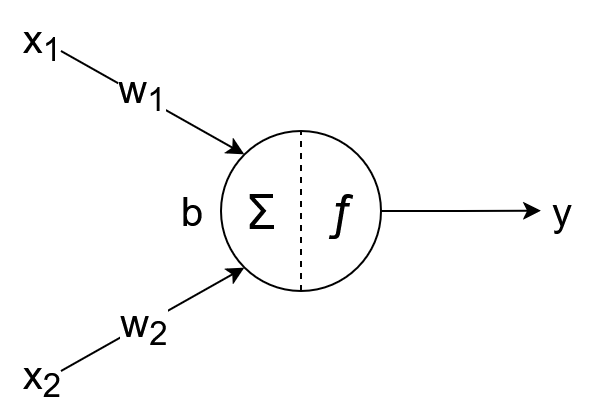
\includegraphics[width=0.7\linewidth]{images/neuron.png}
	\end{center}
	\fonte{o autor}
\end{figure}

No exemplo representado na Figura \ref{fig:neuron}, um neurônio recebe dados de entrada, $x_1$ e $x_2$, e produz uma saída $y$. Para isso, cada entrada é multiplicada por seu respectivo peso, $w_1$ e $w_2$, e somada junto a um termo de viés $b$ -- assim, a equação resultante é igual a $\sum = x_1 w_1 + x_2 w_2 + b$. Finalmente, aplica-se uma função de ativação $f$ sobre a soma para converter esse valor em um intervalo desejado -- a tangente hiperbólica produziria um número dentro do intervalo $(-1, 1)$, enquanto a sigmoide produziria um intervalo entre $(0, 1)$, por exemplo -- resultando na saída $y$ \cite{deeplearningbook}. Em outras palavras, os pesos indicam a importância, ou força, da conexão entre a entrada e o neurônio; o viés atua como um limiar de ativação que independe das entradas; e a função de ativação transforma uma entrada linear em uma saída não linear, o que permite um mapeamento complexo entre entradas e saídas. 

Uma rede neural artificial é formada pela interligação de neurônios, assim, uma camada da rede é denominada a partir de um grupo de nós interligados, que processam dados de uma maneira específica. Combinando uma camada de entrada, camadas intermediárias e uma camada de saída, obtém-se uma rede neural profunda, ilustrada na Figura \ref{fig:dnn}. Dessa forma, cada camada recebe entradas ponderadas a partir das camadas anteriores, aplicam uma função de ativação e propagam o resultado para as camadas subsequentes \cite{deeplearningbook}. Diferentes configurações destas, como a variação das conexões entre neurônios ou o emprego de funções de ativação distintas, tem por efeito especializações, ou habilidades de aprendizado específicas, assim, a utilização de múltiplas camadas permite a assimilação de representações hierárquicas complexas. \cite{reviewdeep}.

\begin{figure}[H]
	\caption{\label{fig:dnn}Representação de um Neurônio Artificial}
    \begin{center}
    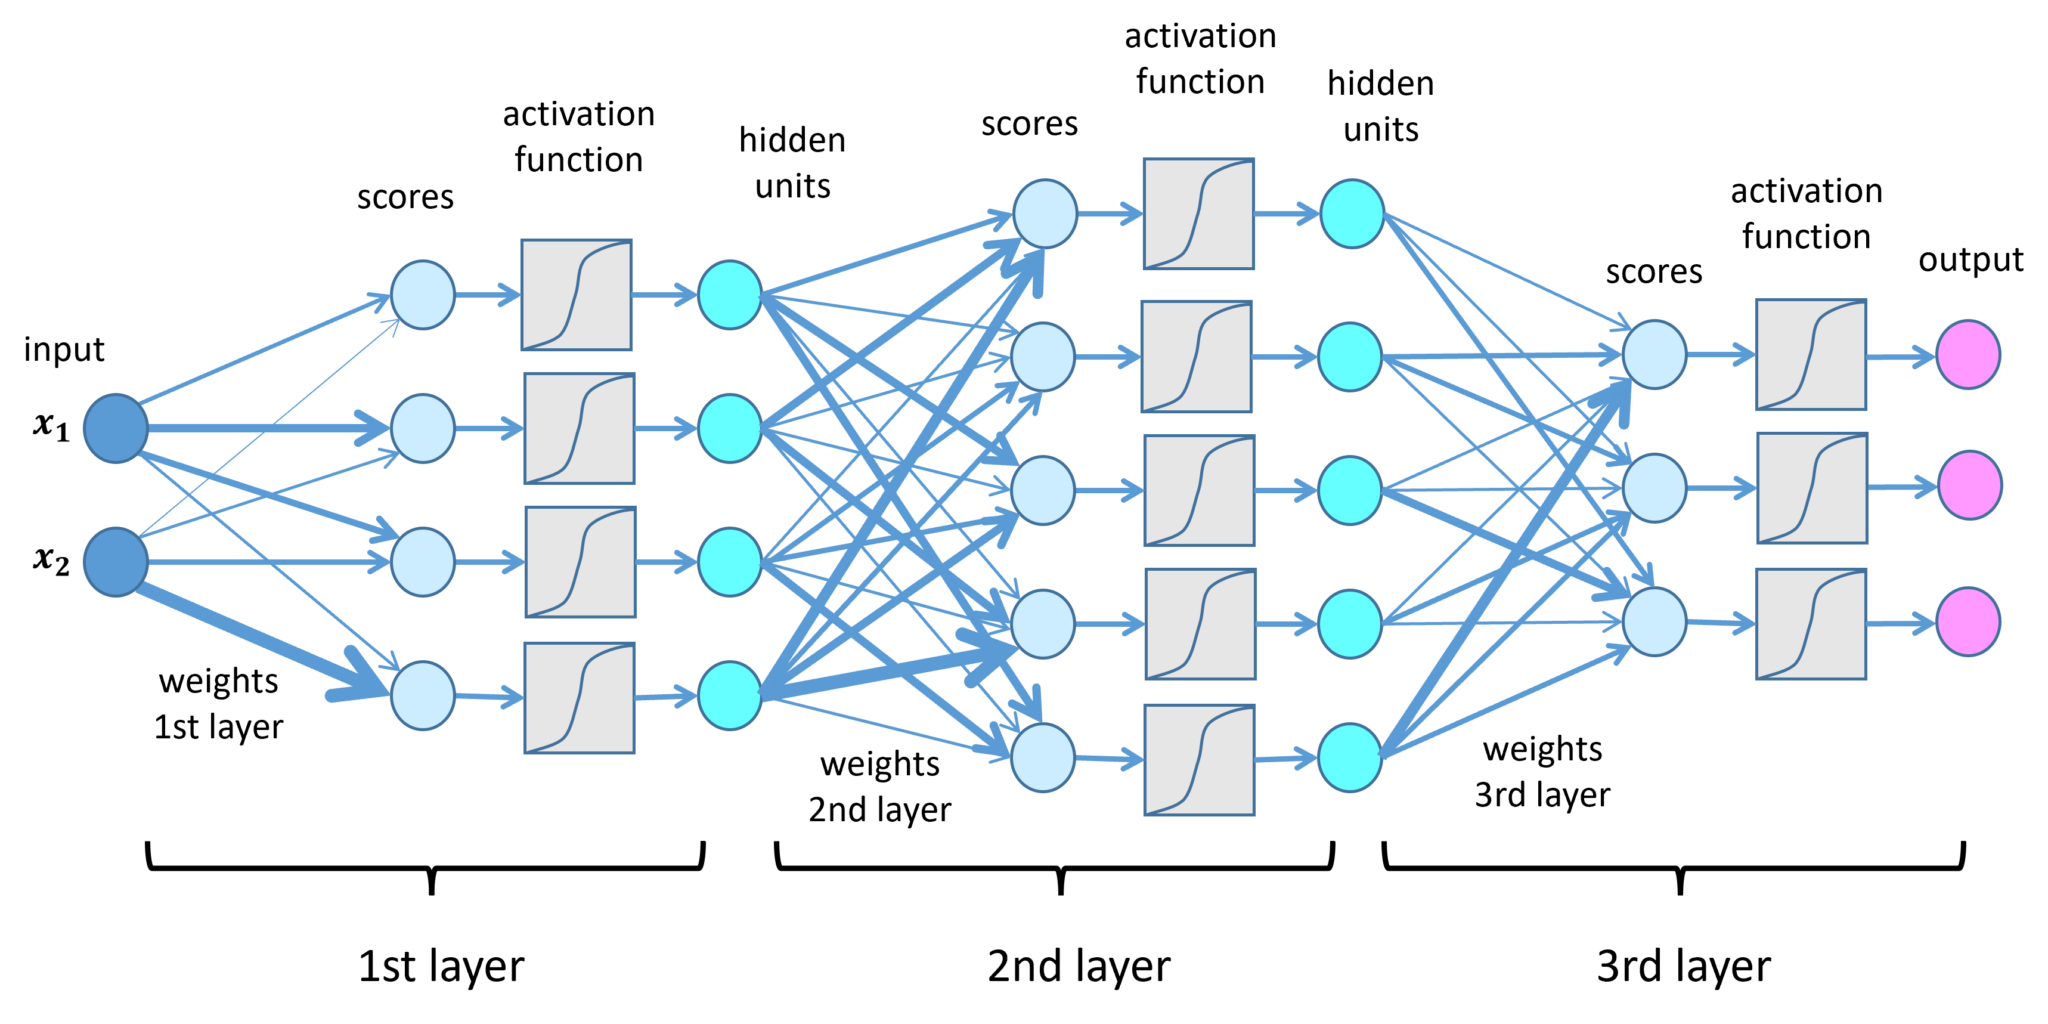
\includegraphics[width=1\linewidth]{images/dnn.png}
	\end{center}
	\fonte{\url{https://lamarr-institute.org/blog/deep-neural-networks/}. Acesso em: 25 junho 2025}
\end{figure}


O processo de aprendizado da rede é denominado treinamento e consiste na estimação e ajuste dos parâmetros através de um algoritmo de retropropagação. Seu objetivo é calcular o gradiente de uma função que mede o erro entre o valor de saída computado e o esperado, além de ajustar os pesos e vieses dos neurônios na direção oposta ao gradiente, para minimizar o erro. Esse processo é executado em cada camada, propagando o erro desde a camada de saída até a de entrada, de forma iterativa, por múltiplas épocas, até que a rede converja para uma solução otimizada \cite{deeplearningbook}, como ilustrado na Figura \ref{fig:gradientdescent}, em que o eixo $y$ representa valores de erro e o eixo $x$ valores de peso.

\begin{figure}[H]
	\caption{\label{fig:gradientdescent}Visualização do Gradiente Descendente}
    \begin{center}
    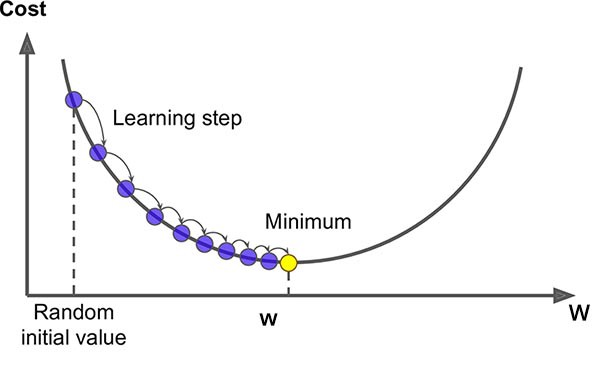
\includegraphics[width=1\linewidth]{images/gradientdescent.jpg}
	\end{center}
	\fonte{\url{https://mlpills.dev/machine-learning/gradient-descent/}. Acesso em: 25 junho 2025}
\end{figure}


\subsection{Redes Neurais Convolucionais}

Redes neurais convolucionais são tipos de redes neurais profundas especialmente úteis na área de visão computacional, especializadas na computação de dados estruturados em topologia de malha, representados matricialmente. O que propicia essa propriedade é o emprego de operações de convolução em pelo menos um módulo da rede, o que consiste em uma mudança no processamento de entrada dos neurônios: ao invés da simples soma ponderada pelos pesos, um cálculo é efetuado a partir da aplicação de um filtro sobre um \textit{input} \cite{deeplearningbook}. Dessa forma, a estrutura de um modelo básico combina camadas convolucionais com camadas de subamostragem, todas esparsamente conectadas \cite{reviewdeep}.

Convolução é uma operação matemática sobre duas funções para a criação de uma terceira, que representa, em termos simplórios, a sobreposição delas. No contexto de redes convolucionais, consiste na multiplicação de duas matrizes seguida de uma soma \cite{origindl}, como demonstrado na Figura \ref{fig:convolution}.

\begin{figure}[H]
	\caption{\label{fig:convolution}Visualização de uma Operação de Convolução}
    \begin{center}
    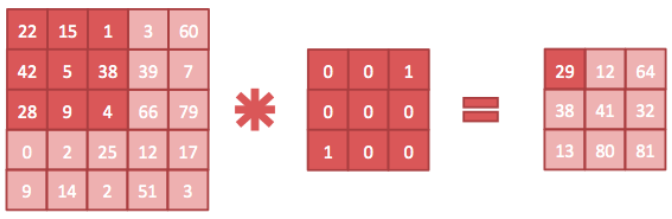
\includegraphics[width=0.75\linewidth]{images/convolution.png}
	\end{center}
	\fonte{\cite{origindl}}
\end{figure}


Um filtro -- ou \textit{kernel}, matrizes de parâmetros aprendíveis -- desliza sobre os dados de entrada, a um passo definido, computando o produto escalar entre seus pesos e os valores correspondentes na região coberta, de forma a criar um mapa de características que representa a presença de padrões específicos detectados pelo filtro \cite{deeplearningbook}. Dessa forma, certas configurações, como o tamanho e os pesos do \textit{kernel}, ou o número de passos de deslizamento, controlam a resolução espacial e a capacidade de modelar relações de vizinhança, como figurativamente representado na Figura \ref{fig:nono}, em que a escolha de um filtro inicial para a detecção de bordas permite o treinamento da rede para a distinção entre gatos magros e gordos.

\begin{figure}[H]
	\caption{\label{fig:nono}Representação da Classificação de uma Imagem por uma Rede Convolucional}
    \begin{center}
    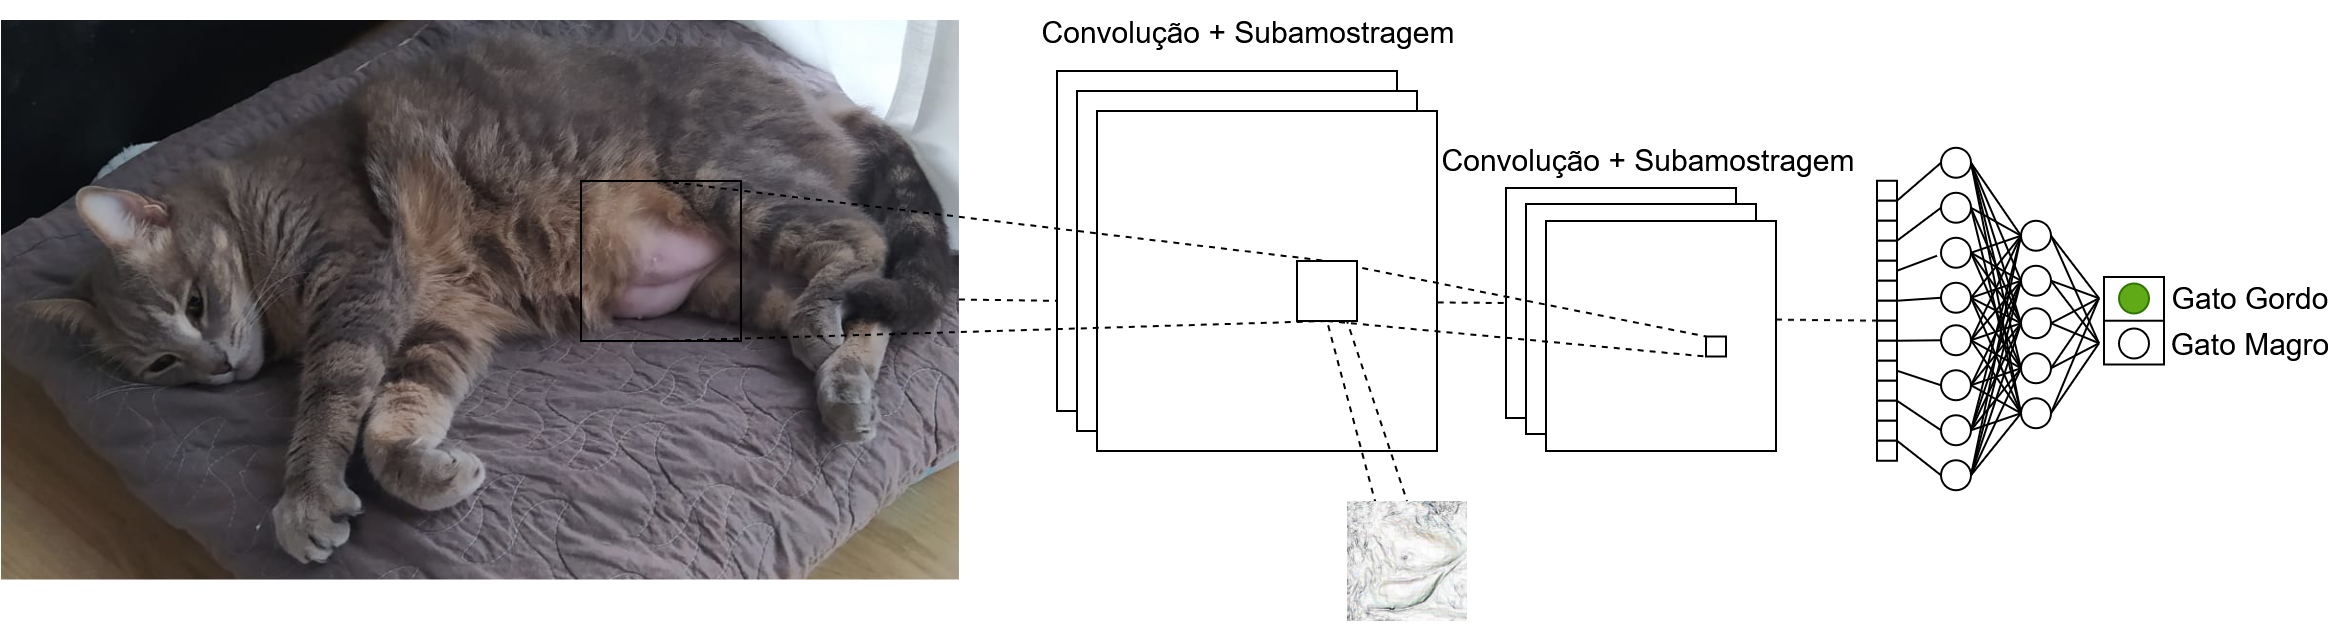
\includegraphics[width=1\linewidth]{images/nono.png}
	\end{center}
	\fonte{o autor}
\end{figure}

Outro importante aspecto das redes convolucionais são as camadas de subamostragem, que reduzem a dimensão espacial dos dados de entrada ao passo em que preservam suas características mais relevantes, processo conhecido como \textit{pooling}. Atingem isso com a obtenção de apenas uma amostra para cada região analisada, para isso, empregam estratégias como \textit{max-pooling} (extração do maior valor de entrada) e \textit{average-pooling} (extração da média dos valores de entrada). A combinação de camadas convolucionais com camadas de subamostragem conferem às essas redes três propriedades fundamentais: a invariância à pequenas transformações, distorções e translações da entrada, que permite que características sejam detectadas independentemente de sua localização; a capacidade de extrair hierarquias espaciais através da redução progressiva de dimensionalidade; e a redução do custo computacional das camadas subsequentes \cite{origindl}.

Dessa forma, a extração de \textit{features} acontece conforme a entrada percorre a rede. Utilizando como exemplo uma imagem para a entrada, as camadas iniciais capturam informações de baixo nível, como bordas, cantos e texturas. Em camadas intermediárias, essas informações passam a compor padrões semânticos locais, como delimitações de objetos, até que, em camadas mais profundas, transformam-se em caracterizações globais de alto nível, como formas completas. Isso permite que as camadas finais possam prever, ou extrair, representações complexas e abstratas \cite{reviewdeep}, como o exemplo utilizado anteriormente -- a classificação entre gatos gordos e magros.

\subsubsection{Reconhecimento Óptico de Caracteres (OCR)}

O reconhecimento óptico de caracteres (OCR), no contexto de computação, descreve um tipo de software que tem por objetivo a conversão de texto, seja impresso ou em imagem, a um formato digital que possa ser processável por máquina \cite{ocr}. É um problema que pode ser tratado utilizando técnicas de segmentação da visão computacional clássica junto a heurísticas, no entanto, as abordagens que utilizam o aprendizado de máquina -- em especial, redes convolucionais -- têm se mostrado mais eficientes e precisas.

De acordo com \citeauthor*{ocr} \cite*{ocr}, um processo de reconhecimento de caracteres moderno tipicamente passa pelo seguinte \textit{pipeline}:

\begin{enumerate}
	\item Aquisição da imagem: obtém-se a imagem com o texto a partir de uma fonte externa, como \textit{scanner} ou câmera;
	\item Pré-processamento: aplicam-se técnicas como remoção de ruído, operações morfológicas e limiarização para melhorar a qualidade da imagem;
	\item Segmentação de caracteres: separam-se os caracteres através da análise de componentes conectados, perfis de projeção ou métodos avançados para tratar textos sobrepostos ou fragmentados;
	\item Extração de \textit{features} e classificação de caracteres: com os caracteres separados, utiliza-se uma rede convolucional para a extração e classificação de seus padrões;
	\item Pós-processamento: para refinar os resultados e aumentar a acurácia, combinam-se técnicas de processamento de linguagem natural, como corretores ortográficos e dicionários com modelos probabilísticos, como cadeias de Markov e N-gramas.
\end{enumerate}

\subsection{Processamento de Linguagem Natural}

O processamento de linguagem natural é um subcampo da inteligência artificial que se dedica ao desenvolvimento de algoritmos capazes de compreender, interpretar e processar linguagem humana de forma computacional. Tradicionalmente, as abordagens baseavam-se em métodos estatísticos, modelos de N-gramas, campos aleatórios condicionais e máquinas de vetores de suporte. Contudo, as últimas décadas têm visto a adoção de técnicas baseadas em redes neurais profundas, que demonstraram capacidade superior de capturar relações complexas entre palavras e compreender contextos linguísticos mais amplos \cite{nlp}.

Fundamentalmente, as técnicas modernas de processamento de linguagem consistem na transformação de texto em representações numéricas que preservam informações sintáticas e semânticas. \textit{Embeddings} de palavras constituem o passo base dessa transformação, que consiste em um mapeamento destas para vetores densos, onde termos semanticamente similares ocupam posições próximas \cite{nlp}. Isso possibilita o aprendizado de estruturas gramaticais e padrões linguísticos, que por sua vez permitem a predição de palavras com base em contextos previamente vistos.

As abordagens modernas de processamento de linguagem dividem-se, majoritariamente, em duas arquiteturas de redes profundas: especializações de redes neurais recorrentes, como LSTM (\textit{long short-term memory}), desenvolvidas para capturar dependências de longo prazo em sequências; ou arquiteturas \textit{Transformers}, capazes do processamento de sequências de forma paralela \cite{nlp2}.

Diferentemente dos modelos de rede apresentados anteriormente, em que os nós processam entradas de maneira independente e passam o resultado adiante, as redes neurais recorrentes utilizam conexões recorrentes, isto é, a saída de um neurônio é retroalimentada à sua camada no próximo passo de processamento, como ilustrado na Figura \ref{fig:rnn}. Essa retroalimentação permite a conservação de um estado oculto que pode ser atualizado a cada passo temporal. Isso permite a captura de padrões e relações temporais dentro de uma sequência, tornando-as boas candidatas ao processamento de texto e outros dados onde a ordenação dos elementos é importante \cite{rnn}. No entanto, apesar de teoricamente capazes de capturar dependências de longo prazo, modelos básicos acabam gradualmente perdendo informações distantes conforme as sequências de entrada ficam longas \cite{nlp}. Isso ocorre por conta do problema de dissipação de gradiente, fenômeno inerente a redes profundas treinadas por \textit{backpropagation}, onde os gradientes utilizados para atualizar os pesos das camadas anteriores diminuem exponencialmente à medida que se retropropagam \cite{deeplearningbook}. Isso significa que as camadas iniciais recebem gradientes muito pequenos, o que resulta em uma atualização insignificante dos pesos e, consequentemente, aprendizado lento ou até mesmo nulo.

\begin{figure}[H]
	\caption{\label{fig:rnn}Representação de uma Rede Neural Recorrente}
    \begin{center}
    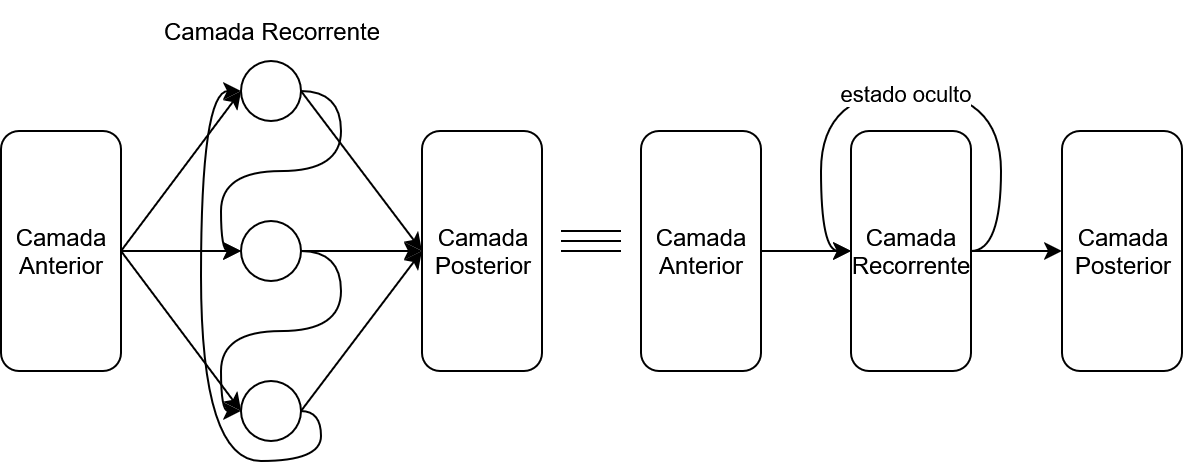
\includegraphics[width=1\linewidth]{images/rnn.png}
	\end{center}
	\fonte{o autor}
\end{figure}

Para resolver essa limitação, as redes LSTM utilizam células que controlam seletivamente o fluxo de informações. Essas estruturas guardam um estado por intervalos de tempo e são compostas, de forma geral, por três mecanismos principais: \textit{forget gates} determinam quais informações devem ser descartadas; \textit{input gates} determinam quais novas informações serão armazenadas no estado da célula; \textit{output gates} determinam quais partes do estado interno influenciarão a saída. Essas decisões são tomadas a partir do cálculo de funções -- tipicamente sigmoide, que resulta em um intervalo entre 0 e 1 -- sobre parâmetros aprendíveis \cite{lstm}. Dessa forma, a rede passa a aprender a lembrar dependências de longo prazo, ou esquecer informações contextuais desnecessárias.

Embora os modelos LSTM sejam eficazes no processamento de texto, possuem uma limitação principal: precisam processar a entrada sequência a sequência -- ou palavra a palavra --, porque a computação dos estados seguintes dependem da computação dos estados anteriores. Isso faz com que o treinamento e a inferência sejam muito lentos e pouco escaláveis \cite{nlp2}.

As arquiteturas \textit{Transformer} superam essa limitação através do processamento paralelo de todos os termos da sequência de entrada. Isso é possibilitado pelas camadas de atenção, que calculam pesos que interconectam diferentes posições do \textit{input}, permitindo que o modelo foque nas palavras mais relevantes às que estão em processamento. Esse processo acontece da seguinte forma: nas camadas iniciais da rede, a sequência de \textit{embeddings} passa por três projeções lineares independentes, de forma a criar, para cada termo, vetores de consultas, chaves e valores; as camadas de atenção então computam similaridades entre as coleções de consulta e de chaves, normalizam esses escores em coeficientes para a obtenção de uma matriz de pesos, e combinam coleções de valores correspondentes de forma ponderada por esses pesos. Assim, operações aplicadas sobre consultas e chaves resultam na obtenção de valores que capturam, em cada posição, as dependências contextuais mais relevantes de toda a sequência -- tudo isso de modo paralelo \cite{transformer}.

Dessa forma, os modelos \textit{Transformer} estruturam-se em duas partes, a primeira consiste na utilização de blocos de codificação, que aplicam sucessivamente camadas de atenção e de propagação comum, assim, esses blocos "prestam atenção" somente na sequência de entrada. A segunda emprega blocos de decodificação que, em relação aos blocos de codificação, adicionam camadas intermediárias de atenção codificador-decodificador. Essas camadas recebem em sua entrada, além da saída das camadas de atenção anteriores, as saídas diretas dos blocos de codificação e, dessa forma, "prestam atenção" tanto na sequência de saída quanto a de entrada. A consequência dessa arquitetura é que o processo de codificação transforma as sequências de entrada em representações abstratas, que incorporam informações de todo o contexto, enquanto a decodificação utiliza essas representações para gerar novos termos de saída, condicionando cada novo elemento tanto às informações abstraídas da entrada quanto ao contexto já produzido pela própria sequência de saída \cite{transformer}.

\section{Análise Multimodal}

A análise multimodal refere-se à integração de informações provenientes de diferentes modalidades de dados, como texto, imagem, áudio e vídeo. Esse tipo de análise reconhece que informações relevantes podem estar distribuídas entre diferentes categorias de dados, sendo que cada uma contribui com aspectos únicos e complementares para a compreensão completa do conteúdo \cite{multimodalsurvey}. Utilizando o caso do presente estudo como exemplo, em um documento acadêmico, o texto isoladamente pode parecer legítimo, no entanto, quando combinado com inconsistências visuais, pode revelar sinais de falsificação, e vice-versa.

No contexto de aprendizado de máquina, o processo conhecido como fusão multimodal consiste em combinar as diferentes representações de tipos de dados em uma unificada, possibilitando que os modelos consigam aprender as características mais relevantes em diferentes domínios de forma prática e eficiente, o que resulta em representações mais ricas e discriminativas \cite{multimodalsurvey,multimodalforgery}. Dessa forma, as estratégias de fusão são normalmente classificadas em quatro categorias principais, dependendo do momento em que ocorrem: fusão precoce, onde as representações brutas são combinadas e servem de entrada para o modelo de aprendizado; fusão intermediária, onde as representações são incorporadas durante as etapas de aprendizado, como em camadas intermediárias de uma rede neural; fusão tardia, onde as decisões de classificadores de modalidades distintas são combinadas; e fusão híbrida, que combina diferentes estratégias de fusão \cite{multimodalsurvey}.

A metodologia deste trabalho utilizará a fusão precoce para combinar os dados extraídos, representados em vetores, a partir das modalidades visuais e textuais. Para isso, \citeauthor*{multimodalmeta} \cite*{multimodalmeta} e \citeauthor*{multimodalforgery} \cite*{multimodalforgery} apresentam diferentes técnicas:

\begin{itemize}
	\item Concatenação básica: abordagem mais simples e direta. Consiste na concatenação simples dos vetores de dados;
	\item Adição elemento a elemento: consiste na soma direta entre os respectivos elementos de cada modalidade;
	\item Transformação bilinear: consiste no produto matricial entre os vetores;
	\item Soma ponderada (\textit{gated summation}): utiliza uma rede neural com funções de ativação específicas, como \textit{weighted sigmoid gate units}, para somar os elementos de forma ponderada, como se o modelo passasse a entender a importância de cada fonte de informação;
	\item Produto ponderado: semelhante à soma ponderada utiliza uma rede neural, mas emprega mecanismos de atenção para o aprendizado, dessa forma, o resultado é o produto matricial entre os vetores, ponderado por uma matriz de pesos.
\end{itemize}

Não existe uma técnica ótima para todos os casos, visto que são subjetivas às características específicas dos domínios ao qual se deseja a união e, assim, a escolha pela melhor abordagem é geralmente determinada pela análise empírica dos resultados \cite{multimodalmeta}.

Além disso, o emprego da fusão multimodal é geralmente associado a outras estratégias auxiliares, que podem tratar tanto os vetores de representação antes da fusão quanto o resultante. Por exemplo, diferentes modalidades possuem características estatísticas e distribuições distintas, dessa forma, pode ser necessário pré-processamento para normalização das escalas dos dados. Da mesma forma, o vetor resultante, por juntar dados muitas vezes situados em espaços de alta dimensionalidade, precisa da aplicação de técnicas de redução dimensional para evitar problemas relacionados à \textit{maldição da dimensionalidade} -- \citeauthor*{bellmancurse} \cite*{bellmancurse} explica que ao lidar com dados em espaços de alta dimensão, sua amostragem e modelagem torna-se progressivamente mais esparsa e difícil dado que o volume do espaço cresce exponencialmente.

\section{Algoritmos de Agrupamento}

No contexto de aprendizado de máquina, as técnicas de agrupamento, ou \textit{clustering}, têm por objetivo a organização de uma coleção de dados em grupos, ou \textit{clusters}, de forma que os elementos dentro de um mesmo grupo tenham muito mais similaridades entre si do que entre elementos em outros grupos. Essas técnicas geralmente são utilizadas quando não se tem conhecimento sobre como os dados podem ser categorizados, dessa forma, tradicionalmente são associadas à aprendizagem não supervisionada \cite{cluster1}. Assim, têm como propósito descobrir estruturações, relações, associações ou hierarquias ocultas dentro da coleção, de maneira a proporcionar melhor compreensão sobre os dados e seus processos subjacentes de criação \cite{cluster2}.

Como trata-se de uma larga área de estudo, os algoritmos de \textit{clustering} variam significativamente em sua compreensão do que constitui um \textit{cluster} e de como este pode ser encontrado de forma eficiente, dessa forma, noções populares incluem grupos com pequenas distâncias entre membros, áreas densas do espaço de dados, intervalos ou distribuições estatísticas específicas \cite{cluster2}. Por fins de brevidade, aqui explicam-se os métodos de agrupamento particional -- que buscam criar grupos a partir do particionamento único da coleção de dados, de forma que um elemento não pertença a mais de um grupo \cite{cluster1} --, em especial, algoritmos baseados em distância e em densidade.

Para os algoritmos baseados em distância, cada \textit{cluster} é representado por um protótipo e a atribuição de elementos a estes é guiada pela minimização de alguma medida de dissimilaridade. Em termos mais concretos, tanto os \textit{clusters} quanto os dados são tipicamente traduzidos como pontos em um espaço. Busca-se então a minimização de uma função de custo, como a soma das distâncias quadráticas entre cada elemento e um \textit{cluster}. Isso acontece através do calculo iterativo da função de custo seguido do ajuste posicional do \textit{cluster}, processo repetido alternadamente até que a valor de custo fique abaixo de um limiar determinado, garantindo a convergência do algoritmo, ou seja, a posição ótima do agrupamento \cite{cluster1, cluster2}.

\begin{figure}[H]
	\caption{\label{fig:kmeans}Representação de um Algoritmo de \textit{Clustering} por Distância}
    \begin{center}
    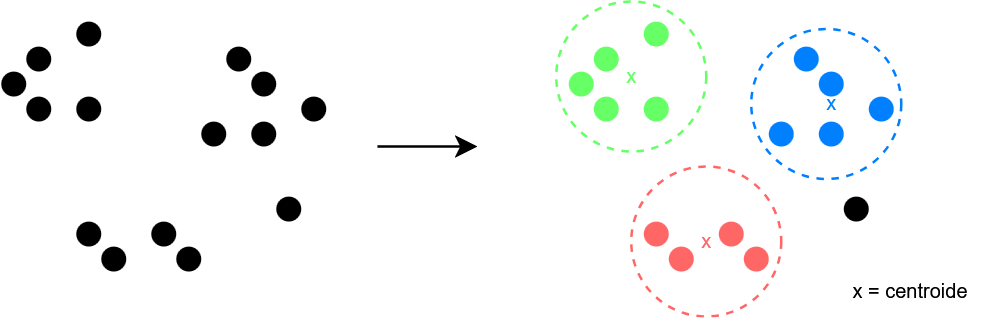
\includegraphics[width=1\linewidth]{images/kmeans.png}
	\end{center}
	\fonte{o autor}
\end{figure}

Os algoritmos baseados em densidade consideram que \textit{clusters} são regiões de alta densidade de dados separadas por áreas de baixa densidade, assim, tanto o formato dos agrupamentos quanto a distribuição dos elementos podem ser feitos de forma arbitrária. O algoritmo DBSCAN pode ser utilizado para exemplificar esse conceito: definem-se os parâmetros $\epsilon$ (raio de vizinhança) e $MinPts$ (número mínimo de pontos ou elementos), assim, um ponto considera outro como vizinho quando está dentro de $\epsilon$. Então, conta-se o número de vizinhos para cada ponto: aqueles com vizinhança densa, isto é, número de vizinhos maior que $MinPts$, tornam-se pontos centrais e formam núcleos de \textit{clusters}; aqueles atingíveis por vizinhança dentro de um \textit{cluster} são absorvidos e chamados de pontos de fronteira; e aqueles pouco densos e não atingíveis são classificados como ruído. \cite{cluster1}.

\begin{figure}[H]
	\caption{\label{fig:dbscan}Representação do Algoritmo DBSCAN}
    \begin{center}
    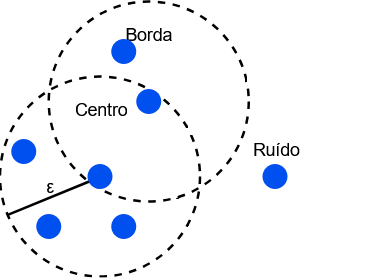
\includegraphics[width=.5\linewidth]{images/dbscan.png}
	\end{center}
	\fonte{o autor}
\end{figure}

\subsection{Detecção de Anomalias}

A detecção de anomalias é definida como o processo de identificar padrões em um conjunto de dados cujo comportamento difere significativamente do esperado, assim, pode ser tratado como um problema de identificação de \textit{outliers} ou ruídos em algoritmos de agrupamento. Quando identificadas, embora nem sempre representem atividades maliciosas, frequentemente indicam eventos de interesse que merecem investigação \cite{anomaly, cluster2}.

A metodologia típica segue três etapas principais: parametrização e pré-processamento, onde os dados são normalizados em formatos comuns; treinamento, onde são construídos modelos de comportamento normal; e finalmente, detecção, em que uma nova observação é comparada aos modelos construídos \cite{anomaly}. Dessa forma, a detecção de anomalias baseada em \textit{clustering} funciona estabelecendo modelos de normalidade através do agrupamento de dados e, posteriormente identificando novos elementos que apresentam desvios expressivos desses modelos de referência.

\chapter{Trabalhos Correlatos}

As próximas seções apresentam os mais recentes trabalhos com temática ou abordagem semelhante.

\section{Visão Geral}

Durante a pesquisa por bibliografia que trata especificamente do problema da identificação de documentos falsificados, foram encontrados poucos resultados, sobretudo no âmbito acadêmico, já que a maioria dos trabalhos com temática similar aborda a classificação de fraudes -- dificuldade ilustrada pela tabela \ref{tab:bibliography}, que apresenta a bibliografia obtida que trata desse tema. É importante distinguir que, a detecção de fraudes foca em adulterações de arquivos originais, como a mudança de notas, datas ou nomes, enquanto a de documentos falsificados busca identificar aqueles completamente forjados desde sua criação, sem terem sido emitidos por instituições oficiais, por exemplo. Isso não significa que as ideias e técnicas não possam ser aproveitadas e adaptadas entre um contexto e outro, pelo contrário, este trabalho de conclusão de curso tem como referência métodos nos dois domínios.

\begin{table}[H]
    \caption{Bibliografia Pesquisada com Temas Abordados}
    \label{tab:bibliography}
    \resizebox{\linewidth}{!}{%
    \begin{tabular}{@{}l|c@{}}
      \toprule
      \multicolumn{1}{c}{Artigos de Detecção de Fraude} & \multicolumn{1}{c}{Aborda Detecção de Falsificação} \\
      \midrule
        \citeauthor*{blockchainforgery} \cite*{blockchainforgery} & \checkmark \\ \hline
        \citeauthor*{clusterfraudverification} \cite*{clusterfraudverification} & \\ \hline
        \citeauthor*{inkcnn} \cite*{inkcnn} & \\ \hline
        \citeauthor*{hashdetection} \cite*{hashdetection} & \\ \hline
        \citeauthor*{multimodalforgery} \cite*{multimodalforgery} & \checkmark \\ \hline
        \citeauthor*{mldocauth} \cite*{mldocauth} & \\ \hline
        \citeauthor*{ocrgraph} \cite*{ocrgraph} & \\ \hline
        \citeauthor*{unsupervisednetwork} \cite*{unsupervisednetwork} & \checkmark \\
      \bottomrule
    \end{tabular}%
  }
\end{table}

Nesta área, é predominante o emprego de estratégias de visão computacional, como o artigo de \citeauthor*{inkcnn} \cite*{inkcnn}, que utiliza \textit{autoencoders} convolucionais para a extração de características em imagens hiperespectrais, focando em identificar incompatibilidade entre tintas. A análise de imagens é frequentemente combinada com técnicas complementares para melhorar a robustez da detecção: \citeauthor*{unsupervisednetwork} \cite*{unsupervisednetwork} propõem uma abordagem não supervisionada que utiliza correlações entre espectros de materiais dos documentos para gerar redes ponderadas, aplicando algoritmos de \textit{clustering} para identificar padrões anômalos; \citeauthor*{ocrgraph} \cite*{ocrgraph} introduziram outra perspectiva ao reformular o problema como comparação de grafos, em que obtém, via OCR, caixas delimitadoras de tamanho entre caracteres, utilizando-as para o treinamento de classificadores que detectam a manipulação de \textit{pixels}.

Alternativamente, também existem propostas que abordam a prevenção de fraudes através de outras tecnologias, como \citeauthor*{hashdetection} \cite*{hashdetection}, que propõe o emprego de funções criptográficas para detectar modificações em documentos previamente submetidos, em que são armazenados os valores de \textit{hash} dos arquivos originais e legítimos, de forma que validações posteriores possam ser comparadas com o certificado primário. Contudo, essas abordagens preventivas não lidam com a classificação de documentos falsificados em sua concepção, representando uma lacuna pouco explorada, que o presente estudo visa preencher. Em sequência seguem os trabalhos que guiaram a concepção da estratégia da presente pesquisa.

\section{``\protect\textit{Blockchain Smart Contract to Prevent Forgery of Degree Certificates: Artificial Intelligence Consensus Algorithm}``}

Para o problema de prevenção de fraudes de diplomas, o artigo de \citeauthor*{blockchainforgery} \cite*{blockchainforgery} propõe uma \textit{blockchain} que incorpora algoritmos de aprendizado de máquina em diversas partes do processo de verificação de documentos e de consenso da rede. Além disso, de forma semelhante ao trabalho de \citeauthor*{hashdetection} \cite*{hashdetection}, quando um certificado é aceito, seu \textit{hash} é calculado e integrado ao seu registro na rede, permitindo sua verificabilidade, de forma que qualquer adulteração seja facilmente detectada.

O autor apresenta o fluxo para submissão de um diploma na \textit{blockchain} em quatro etapas principais, conforme Figura \ref{fig:blockchainforgery}.

\begin{figure}[H]
	\caption{\label{fig:blockchainforgery}Representação da Arquitetura de Validação de Diplomas por \citeauthor*{blockchainforgery}}
    \begin{center}
    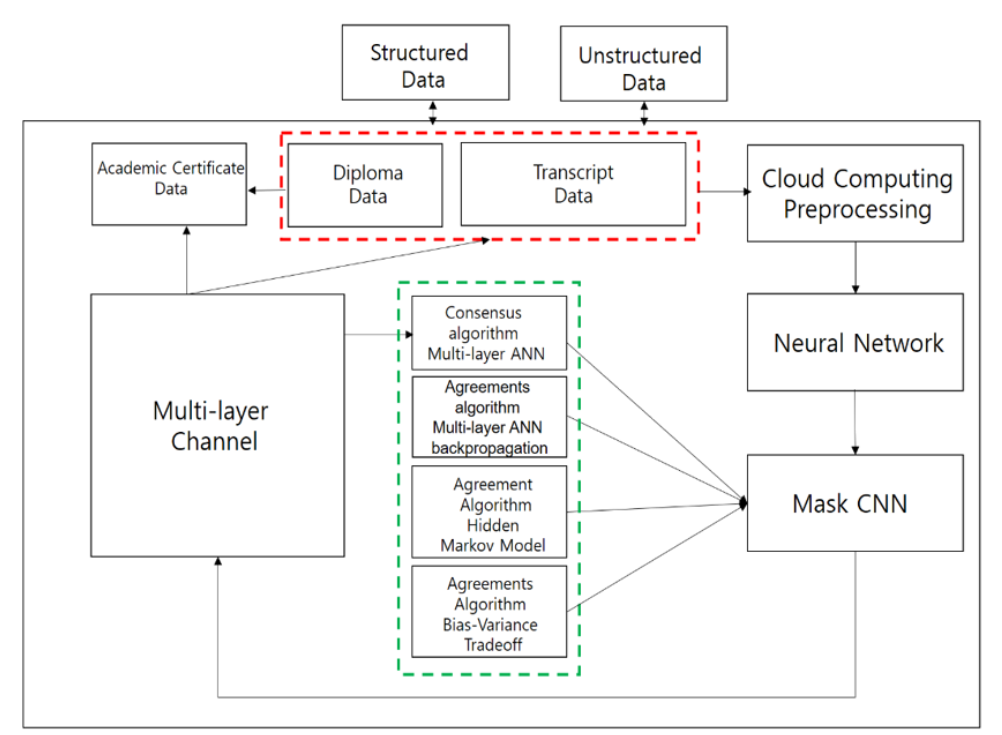
\includegraphics[width=1\linewidth]{images/blockchainforgery.png}
	\end{center}
	\fonte{\cite{blockchainforgery}}
\end{figure}
 
A primeira etapa, "\textit{Cloud Computing Preprocessing}", consiste na entrada e pré-processamento do documento digitalizado e, através de um serviço em nuvem, normaliza os dados brutos da imagem, extrai metadados -- como resolução, dimensões e contraste --, aplica correções de perspectiva e cria uma versão virtualizada semi-persistente do arquivo, preparada para ser processada pelas etapas conseguintes, rejeitando entradas com formato e qualidade inconsistentes.

Em seguida, as imagens passam pela etapa "\textit{Neural Network}", que utiliza \textit{Faster R-CNN} para rapidamente filtrar e detectar artefatos visuais suspeitos. Através de sua rede de propostas regionais (\textit{Region Proposal Network}), o algoritmo captura regiões de interesse -- como selos da universidade, assinaturas, marcas d'água e outros padrões -- e cria escores de confiança para cada uma, identificando áreas possivelmente adulteradas.

Os documentos passam então para a etapa "\textit{Mask CNN}", que através de um modelo \textit{Mask R-CNN} e das regiões de interesse previamente identificadas, segmenta a imagem, criando máscaras binárias a nível de \textit{pixel}, ou seja, para cada região, o algoritmo estima quais \textit{pixels} pertencem ao document legítimo e quais foram forjados. Essas máscaras são então encapsuladas como prova imutável dentro do bloco que será registrado na blockchain, além de servir como outra medida de escore de confiança do documento.

Por fim, ambas as pontuações de confiança são combinadas e passadas ao mecanismo de consenso dessa \textit{blockchain}, representado pela etapa "\textit{Multi-layer Channel}" que, ao invés de utilizar estratégias tradicionais como prova de trabalho ou prova de participação, combina múltiplos algoritmos de aprendizado de máquina. De forma geral, essa arquitetura é composta por quatro componentes principais:

\begin{itemize}
    \item Um algoritmo baseado em uma rede neural multicamadas, que processa os escores de confiança fornecidos pelos processamentos anteriores e, a partir de certo limiar de confidência, imediatamente aprova o documento;
    \item Um algoritmo de aprendizado complementar à rede neural multicamadas, que cruza referências com padrões aprendidos de decisões anteriores -- por exemplo, quando um diploma inicialmente validado como autêntico posteriormente se prova fraudulento -- e ajusta os pesos da rede;
    \item Um algoritmo que utiliza um modelo oculto de Markov para, a partir de uma cadeia de regras, examinar padrões temporais e fornecer avaliações probabilísticas da autenticidade do documento;
    \item Um algoritmo que equilibra a complexidade (\textit{overfitting}) com a generalização (\textit{underfitting}) do modelo de rede neural, ou seja, procura encontrar \textit{trade-off} ótimo entre viés e variância para decisões de consenso confiáveis.
\end{itemize}

Assim, cada nó da \textit{blockchain} executa esses algoritmos e vota, com base na ponderação dos resultados, se devem incluir ou rejeitar o bloco com o diploma. Para qualquer decisão, exige-se quórum de pelo menos $2/3$ de votos. Caso não seja atingido, seja por discordâncias das máscaras ou pela recusa de validadores de alta reputação, uma nova rodada de votação é iniciada com a reexecução das etapas "\textit{Mask CNN}" e "\textit{Multi-layer Channel}" com parâmetros ajustados. Esse ciclo se repete até obter consenso ou direcionar o diploma a uma auditoria humana. Dessa forma, quando um documento é aprovado na rede, é classificado como autêntico no \textit{ledger}; quando reprovado, é sinalizado como fraudulento.

Por fim, quando um terceiro -- como empresa, universidade ou empregador -- deseja verificar a validade de um diploma já registrado, basta a verificação do \textit{hash} do documento já submetido.

\section{``\protect\textit{Multimodal Document Image Classification}``}

O trabalho de \citeauthor*{multimodal} \cite*{multimodal} não lida diretamente com a identificação de documentos falsificados ou fraudados, mas sim do problema geral de classificação de imagens. No entanto, a abordagem utilizada pelos autores é altamente relevante, pois mostra a eficácia da análise multimodal e pode ser aproveitada por este trabalho de conclusão de curso.

O \textit{paper} propõe uma abordagem multimodal para a classificação de imagens de documentos diversos em dezesseis categorias utilizando o \textit{dataset} RVL-CDIP. A proposta combina a fusão de características visuais e textuais para a rotulagem entre imagens e classes. Para isso, segue o \textit{pipeline}:

\begin{enumerate}
    \item Pré-processamento: normaliza e redimensiona as imagens para utilizações posteriores;
    \item Extração de texto: utiliza OCR para extrair texto das páginas;
    \item Extração multimodal, em paralelo:
    \subitem Modalidade textual: utiliza um modelos de linguagem para capturar informações semânticas dos textos extraídos;
    \subitem Modalidade visual: extrai características das imagens a partir de uma rede convolucional;
    \item Fusão multimodal: combina as extrações textuais e visuais;
    \item Classificação final: utiliza uma rede convolucional, que tem como entrada a fusão multimodal, para classificar os documentos.
\end{enumerate}

Para a modalidade textual, os autores trazem à tona o problema de que texto extraído por OCR pode ser muito ruidoso, contendo erros a nível de caracteres ou até palavras. Por isso, capturam representações do conteúdo em três diferentes granularidades. 

A nível de sequência, empregam ULMFiT (\textit{Universal Language Model Fine-tuning}), um modelo que processa o documento como uma sequência de palavras e mantém uma "memória interna", que armazena informações contextuais conforme processa cada palavra sequêncialmente. Isso permite que a rede neural capture sequências lógicas, dependências de longo prazo e contexto semântico entre palavras distantes. Como saída, o algoritmo produz uma representação vetorial do texto que leva em consideração as características citadas.

A nível de palavra, para representar cada uma, empregam FastText \textit{embeddings}. A técnica consiste em transformar os termos em vetores numéricos, de forma que palavras com significados similares fiquem próximas no espaço matemático. O vetor final do documento é calculado como a média dos \textit{embeddings} de todas as palavras presentes.

A nível de caractere, para capturar padrões ortográficos, aplicam N-gramas de caracteres -- sequências contínuas de n caracteres abduzidos de uma palavra -- e criam um vetor numérico normalizado das ocorrências dos padrões obtidos.

Em resumo, as características de sequência preservam o contexto semântico geral do documento, as representações de palavra mantêm similaridades semânticas locais, e os N-gramas de caracteres oferecem robustez contra erros de OCR e palavras desconhecidas. Essas três representações são combinadas através de um método \textit{ensemble}, que produz um vetor unificado que comporta essas \textit{features} textuais.

Para a modalidade visual, o trabalho emprega a arquitetura de rede VGG-16 (\textit{Visual Geometry Group}) para extrair características hierárquicas através de suas camadas convolucionais, capturando padrões de layout, tipografia, elementos gráficos e padrões de formatação presentes nos documentos. Como saída, a rede produz um vetor multidimensional que representa uma codificação densa e compacta de todas as informações visuais relevantes do documento.

O principal interesse desse trabalho é a fusão das informações textuais e visuais, que tem por objetivo criar uma representação unificada, que preserve e potencialize as informações complementares de ambas as modalidades, e que permita que um modelo de classificação final explore sinergias entre essas diferentes características. Os autores propõem duas estratégias principais para combinar essas representações, das quais destaca-se a segunda, que combina os vetores anteriormente extraídos.

Essa abordagem explora quatro métodos distintos de junção. De forma geral, o primeiro é a concatenação simples, onde os vetores de características textuais e visuais são diretamente concatenados para formar um vetor unificado. O segundo método utiliza adição elemento a elemento, somando diretamente as representações de ambas as modalidades. O terceiro emprega \textit{compact bilinear pooling}, uma técnica mais sofisticada que calcula o produto externo entre os vetores de características para capturar interações complexas entre as modalidades, permitindo que o modelo de classificação posterior aprenda correlações não-lineares entre informações visuais e textuais. Por fim, o quarto método implementa \textit{multimodal gated units}, que utilizam mecanismos de atenção para aprender uma função de controle que determina automaticamente como ponderar e combinar as características de cada modalidade, o que permite que o modelo posterior adapte dinamicamente a importância relativa de informações visuais ou textuais dependendo do contexto específico do documento -- para documentos altamente textuais como contratos ou relatórios científicos, as características semânticas podem ser mais discriminativas, enquanto para documentos com layouts visuais distintivos como formulários ou apresentações, as características visuais podem ser mais relevantes.

Em sequência, para realizar a classificação final, os autores utilizam uma camada densa e uma camada final \textit{softmax} para a predição, como ilustra a Figura \ref{fig:multimodal}.

\begin{figure}[H]
	\caption{\label{fig:multimodal}Representação da Arquitetura de Fusão Multimodal por \citeauthor*{multimodal}}
    \begin{center}
    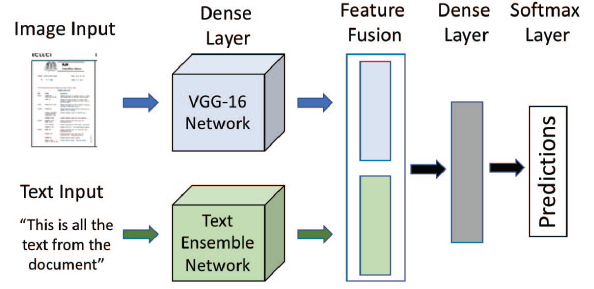
\includegraphics[width=1\linewidth]{images/multimodal.png}
	\end{center}
	\fonte{\cite{multimodal}}
\end{figure}

Finalmente, o artigo compartilha as conclusões finais, onde explicita como essa abordagem superou consistentemente os métodos que utilizam apenas uma modalidade, com o método de adição elemento a elemento curiosamente alcançando os melhores resultados para a fusão multimodal, atingindo uma acurácia de 93,6\% no \textit{dataset} RVL-CDIP.

\section{``\protect\textit{CERTIFICATE FRAUD VERIFICATION MODEL USING CLUSTERED-BASED CLASSIFICATION APPROACH}``}

O trabalho de \citeauthor*{clusterfraudverification} \cite*{clusterfraudverification} lida diretamente com o problema de verificação da autenticidade de certificados acadêmicos. Para isso, propõe uma abordagem baseada em \textit{clustering}, fundamentado na premissa de que documentos legítimos apresentam padrões consistentes de características que podem ser identificados através desses agrupamentos.

O \textit{dataset} utilizado pelos autores consiste em mais de vinte e quatro mil amostras de documentos não rotulados, oficialmente emitidos por duas universidades: Enugu State University of Science and Technology e University of California Irvine.

A metodologia dos autores utiliza o algoritmo K-means como técnica principal para descobrir os padrões dominantes em certificados acadêmicos. Dessa forma, o processo de treinamento consiste na aplicação desse algoritmo sobre as características extraídas dos documentos do \textit{dataset}, com o objetivo de agrupá-los em dezesseis grupos. O algoritmo inicializa centroides e atribui iterativamente cada arquivo ao centroide mais próximo usando um modelo de equidistância. Os centroides são atualizados através do cálculo das médias dos pontos pertencentes a cada \textit{cluster} até atingir convergência. Para a verificação de documentos, o sistema extrai suas características e calcula distâncias em relação aos centroides estabelecidos, classificando-o como legítimo, quando próximo de algum padrão conhecido, ou suspeito, quando distante de todos os \textit{clusters}.

Embora os autores não especifiquem os processos de extração de características, as figuras apresentadas sugerem fortemente o uso de \textit{features} visuais. As imagens, como exemplificado na Figura \ref{fig:clusterfraudverification}, mostram marcações circulares em pontos específicos dos certificados, destacando elementos como logos institucionais e aspectos estruturais dos documentos. Assume-se, portanto, que o sistema captura e converte essas informações em vetores numéricos compatíveis com o K-means.

\begin{figure}[H]
	\caption{\label{fig:clusterfraudverification}Resultado da Verificação de um Documento Autêntico}
    \begin{center}
    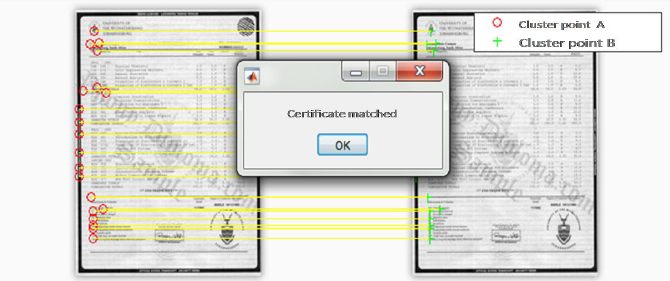
\includegraphics[width=1\linewidth]{images/clusterfraudverification.png}
	\end{center}
	\fonte{\cite{clusterfraudverification}}
\end{figure}

O modelo foi validado experimentalmente com certificados reais e demonstrou capacidade de distinguir documentos autênticos de falsificados, já que os resultados reportaram uma acurácia geral de 86,53\%. Os autores destacam como principal vantagem a capacidade do sistema de operar efetivamente com \textit{datasets} limitados, característica importante em cenários reais onde a disponibilidade de dados rotulados é restrita por questões éticas e de privacidade.

\chapter{Metodologia}

Este capítulo define, de forma preliminar, a metodologia que será seguida durante o desenvolvimento do trabalho e está sujeita a mudanças conforme coleta e análise dos documentos acadêmicos.

\section{Visão Geral da Metodologia}

A metodologia proposta tem como base uma abordagem de aprendizado não-supervisionado e detecção de anomalias através da análise e extração multimodal. Busca-se rotular documentos com base em um nível de probabilidade de fraudulência, para isso, utilizam-se extrações de características visuais (como textura, fonte, espaçamento, selos e assinaturas), textuais (como padrões linguísticos, formatação de números e distribuição de termos) e estruturais (como posição de campos, margens e tabelas), que serão refinadas conforme realização do TCC. Combinando essas \textit{features} multidimensionais, é possível realizar o agrupamento dos documentos em \textit{clusters} que representam padrões dominantes normais. Em sequência, modelos de detecção de anomalias são utilizados para a criação de detectores de referência a partir dos \textit{clusters}, possibilitando a classificação de um novo documento submetido, em tempo real, através da avaliação do grau de desvio em relação aos padrões aprendidos — quanto maior o desvio e escore de anomalia, maior a probabilidade de que o documento seja falsificado. Finalmente, essa pontuação é mapeada para categorias discretas de suspeita, fornecendo um nível de probabilidade de fraude para cada inserção. O processo completo consiste em duas etapas: treinamento dos modelos de referência e classificação de novos documentos.

A escolha dessa abordagem tem por base a premissa de que documentos falsificados apresentam inconsistências sutis, tornando-os atípicos em relação aos padrões estabelecidos por documentos legítimos, sendo detectáveis através da análise multimodal das características extraídas de diversos contextos.

\subsection{Treinamento dos Modelos de Referência}

Representada na Figura \ref{fig:fluxotreino}, a fase de treinamento inicia com a coleta de certificações acadêmicas diversas, seguida do pré-processamento através de técnicas de normalização de imagens e aplicação de OCR. Com o \textit{dataset} formado, é realizada a extração e processamento multimodal de características visuais, textuais e estruturais dos documentos. Em sequência, com base nos dados obtidos na etapa anterior, é realizada a identificação de padrões utilizando algoritmos de \textit{clustering} para identificar grupos de documentos com comportamentos similares, estabelecendo padrões dominantes de normalidade. Por fim, detectores de anomalias são treinados para cada padrão descoberto, gerando modelos de referência normais.

\begin{figure}[H]
	\caption{\label{fig:fluxotreino}Representação do Fluxo de Treino}
    \begin{center}
    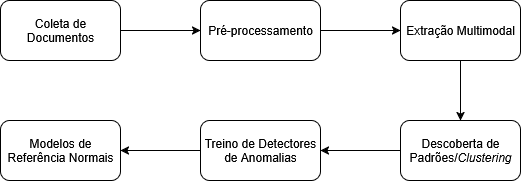
\includegraphics[width=.9\linewidth]{images/FluxoTreino.png}
	\end{center}
	\fonte{o autor}
\end{figure}

\subsection{Classificação de Novo Documento}

Representada na Figura \ref{fig:fluxoanalise}, o processo de classificação de novo documento utiliza os modelos de referência estabelecidos na fase de treinamento para determinar a probabilidade de falsificação.

\begin{figure}[H]
	\caption{\label{fig:fluxoanalise}Representação do Fluxo de Análise de Novo Documento}
    \begin{center}
    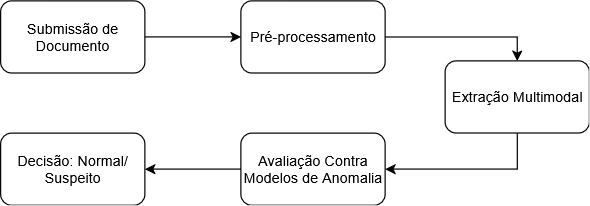
\includegraphics[width=.9\linewidth]{images/FluxoAnalise.png}
	\end{center}
	\fonte{o autor}
\end{figure}

O processo inicia com a submissão de um novo certificado e, para garantir consistência na representação das características, passa pelo mesmo \textit{pipeline} de pré-processamento e extração multimodal utilizado na fase de treinamento. Em seguida, os dados de representação do documento, obtidos na etapa anterior, são comparados contra todos os modelos de referência normal. Cada modelo calcula um escore de anomalia baseado na distância, ou similaridade, em relação ao padrão estabelecido pelo modelo. Essas pontuações representam, por fim, a probabilidade de falsificação do registro. Finalmente, utilizam-se métricas de consenso para categorizar o arquivo, isto é, classificá-lo como normal ou suspeito a partir de determinado limiar de pontos.

\subsection{Extração Multimodal de Características}

O módulo de extração multimodal, utilizado tanto no fluxo de treino quanto no fluxo de classificação de uma submissão, é responsável por capturar diferentes aspectos dos documentos. Essa abordagem permite aproveitar o mesmo \textit{pipeline} de processamento combinando características independentes e, no contexto deste trabalho, complementares. Busca-se poder detectar tanto falsificações grosseiras quanto sofisticadas, uma vez que mesmo contrafações bem-feitas tendem a apresentar inconsistências sutis.

\begin{figure}[H]
	\caption{\label{fig:fluxomultimodal}Representação do Fluxo de Extração Multimodal de Características}
    \begin{center}
    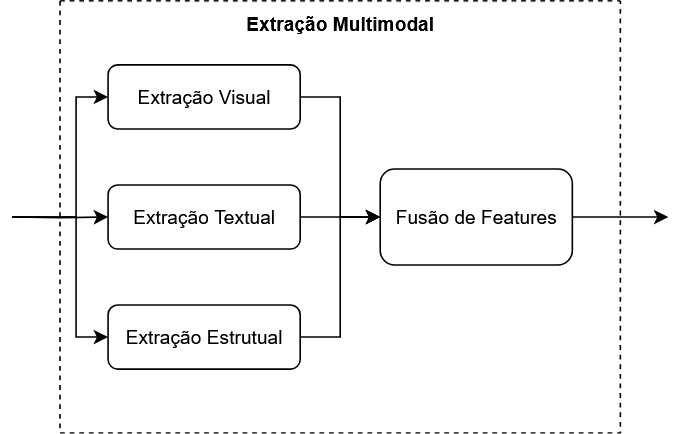
\includegraphics[width=1\linewidth]{images/FluxoExtracao.png}
	\end{center}
	\fonte{o autor}
\end{figure}

Ao invés de focar em características de domínios específicos, como nos trabalhos correlatos, essa abordagem combina três diferentes subprocessos de extração de \textit{features} em paralelo, como representado na Figura \ref{fig:fluxomultimodal}:

\begin{itemize}
    \item Extração visual: extrai características ligadas ao layout, qualidade e consistência visual dos documentos. Inclui análise de textura, propriedades de fonte (espessura, tamanho, espaçamento), qualidade de assinaturas e selos, resolução de imagem, e padrões de cores e contrastes;
    \item Extração textual: utiliza modelos de processamento de linguagem natural para extrair características linguísticas e de formatação. Analisa padrões textuais, distribuição de termos, consistência na formatação de números, datas e códigos, além de verificar a coerência semântica do conteúdo;
    \item Extração estrutural: extrai características ligadas à organização espacial e estrutural dos documentos. Examina posicionamento de campos, formatação de tabelas, alinhamentos, margens, espaçamentos e a disposição geral dos elementos no documento.
\end{itemize}

Por fim, é realizada a fusão das características extraídas em todos os subprocessos. Para isso, os dados são normalizados e são aplicadas técnicas de redução dimensional, evitando a \textit{maldição da dimensionalidade}, o que resulta em uma representação completa, unificada e compacta de cada documento.

\chapter{Próximos Passos}

\section{Cronograma}

A seguir, segue o cronograma planejado para a próxima etapa do projeto e a disciplina de Trabalho de Conclusão de Curso 2.

\begin{table*}[htb]
    \centering\caption{Cronograma para TCC2.}
    \label{tab:cronograma}\resizebox{\textwidth}{!} {
        \rowcolors{0}{shadecolor}{shadecolor}
        \begin{tabular}{|X p{5cm}|c|c|c|c|c|c|c|}
            \hline
            %\multirow{2}{*}{\cellcolor{shadecolor}} \\
            \multirow{-1}{*}{Etapas} &
            \multicolumn{7}{|c|}{2025} \\ \hhline{|~|*{7}{-|}}
            & Ago & Set & Out & Nov & Dez \\ \hline
            
            \hiderowcolors Obtenção e análise dos documentos acadêmicos & X & X & & & \\ \hline
            \hiderowcolors Desenvolvimento do \textit{software} & & X & X & X & \\ \hline
            \hiderowcolors Escrita da monografia & & & & X & X \\ \hline
            \hiderowcolors \textbf{Entrega TCC II} & & & & & X \\ \hline
            \hiderowcolors \textbf{Defesa pública} & & & & & X \\ \hline
        \end{tabular}
    }
\end{table*}

% ----------------------------------------------------------
% ELEMENTOS PÓS-TEXTUAIS
% ----------------------------------------------------------
\postextual
% ----------------------------------------------------------

% ----------------------------------------------------------
% Referências bibliográficas
% ----------------------------------------------------------
\begingroup
	\SingleSpacing
	\printbibliography[title=REFERÊNCIAS]
\endgroup

% ----------------------------------------------------------
% Glossário
% ----------------------------------------------------------
%
% Consulte o manual da classe abntex2 para orientações sobre o glossário.
%
% \glossary

% ----------------------------------------------------------
% Apêndices
% ----------------------------------------------------------

% ---
% Inicia os apêndices
% ---
%\begin{apendicesenv}
%	\partapendices* 
%	% ----------------------------------------------------------
\chapter{Descrição}
% ----------------------------------------------------------

Textos elaborados pelo autor, a fim de completar a sua argumentação. Deve ser precedido da palavra APÊNDICE, identificada por letras maiúsculas consecutivas, travessão e pelo respectivo título. Utilizam-se letras maiúsculas dobradas quando esgotadas as letras do alfabeto. 

\begin{quadro}[htb]
	\centering
	\caption{\label{qua:Quadro_2}Modelo A.}	
\begin{tabular}{|l|l|}
\hline
xxxx              & yyyyyyyyyyyyyyy    \\
\hline
xxxx              & yyyyyyyyyyyyyyy    \\
\hline
xxxx              & yyyyyyyyyyyyyyy    \\
\hline
xxxx              & yyyyyyyyyyyyyyy    \\
\hline
xxxx              & yyyyyyyyyyyyyyy    \\
\hline
xxxx              & yyyyyyyyyyyyyyy    \\
\hline
xxxx              & yyyyyyyyyyyyyyy    \\
\hline
rrrrrrrrrrrrrrrrr & eeeeeeeeeeeeeeeee  \\
\hline
xxxx              & yyyyyyyyyyyyyyy    \\
\hline
xxxx              & yyyyyyyyyyyyyyy    \\
\hline
rrrrrrrrrrrrrrrrr & eeeeeeeeeeeeeeeee  \\
\hline
xxxx              & yyyyyyyyyyyyyyy    \\
\hline
                  & ttttttttttttttttt  \\
\hline
rrrrrrrrrrrrrrrrr & eeeeeeeeeeeeeeeee  \\
\hline
ttttttttttttt     &                    \\
\hline
rrrrrrrrrrrrrrrrr & eeeeeeeeeeeeeeeee  \\
\hline
rrrrrrrrrrrrrrrrr & eeeeeeeeeeeeeeeee  \\
\hline
                  & gggggggggggggggggg \\
\hline
rrrrrrrrrrrrrrrrr & eeeeeeeeeeeeeeeee  \\
\hline
rrrrrrrrrrrrrrrrr & eeeeeeeeeeeeeeeee  \\
\hline
rrrrrrrrrrrrrrrrr & eeeeeeeeeeeeeeeee  \\
\hline
rrrrrrrrrrrrrrrrr & eeeeeeeeeeeeeeeee  \\
\hline
\end{tabular}
\fonte{Elaborada pelo autor (2016).}
\end{quadro}
%\end{apendicesenv}
% ---


% ----------------------------------------------------------
% Anexos
% ----------------------------------------------------------

% ---
% Inicia os anexos
% ---
%\begin{anexosenv}
%	\partanexos*
	%% ----------------------------------------------------------
\chapter{Declaração padrão para empresa ou laboratório}
% ----------------------------------------------------------
	\begin{snugshade}

	\begin{center}
	{\textbf{DECLARAÇÃO DE CONCORDÂNCIA COM AS CONDIÇÕES PARA O DESENVOLVIMENTO DO TCC NA INSTITUIÇÃO}}
	\end{center}
		
	\end{snugshade}

	\vspace{10pt}

	Declaro estar ciente das premissas para a realização de Trabalhos de Conclusão de Curso (TCC) de Ciência da Computação e Sistema de In\-for\-ma\-ções da UFSC, particularmente da necessidade de que se o TCC envolver o desenvolvimento de um software ou produto específico (ex: um protocolo, um método computacional, etc.) o código fonte e/ou documentação completa correspondente deverá ser entregue integralmente, como parte integrante do relatório final do TCC. 

	Ciente dessa condição básica, declaro estar de acordo com a realização do TCC identificado pelos dados apresentados a seguir.

	\vspace{20pt}


	%\noindent\resizebox{\textwidth}{!}{
		\begin{tabular}{|l|X p{8cm}|}
			%\begin{small}
				\hline
			     \textbf{Instituição} &  ECL/INE/CTC \\ \hline
			     \textbf{Nome do Responsável} &  José Luís A. G{\"u}ntzel \\ \hline
			     \textbf{Cargo/Função} &  Prof. INE/CTC \\ \hline
			     \textbf{Fone de Contato} &  (48) 37216466 / (53) 999711982 \\ \hline
			     \textbf{Acadêmico} & Arthur João Lourenço \\ \hline
			     \textbf{Título do trabalho} & Otimização do Roteamento de Circuitos VLSI por meio de Movimentação de Células
de células \\ \hline
			     \textbf{Curso} & Ciências da Computação/INE/UFSC \\ \hline

			%\end{small}
		\end{tabular}
	%}

	\vspace{40pt}

	\begin{flushright}

		Florianópolis, \today.
		
	\end{flushright}

	\vspace{20pt}


	\begin{center}
	    \parbox{7cm}{
	    \centering
	      \rule{6cm}{1pt}\\
	       \small \textbf{Professor Responsável}\\
	       Prof. Dr. José Luís Almada G{\"u}ntzel     
	    }
		\hfill
	\end{center}  



%São documentos não elaborados pelo autor que servem como fundamentação (mapas, leis, estatutos). Deve ser precedido da palavra ANEXO, identificada por letras maiúsculas consecutivas, travessão e pelo respectivo título. Utilizam-se letras maiúsculas dobradas quando esgotadas as letras do alfabeto. 

%\end{anexosenv}

%---------------------------------------------------------------------
% INDICE REMISSIVO
%---------------------------------------------------------------------
%\phantompart
%\printindex
%---------------------------------------------------------------------

\end{document}
